%% 
%% Brody spacing statistics of surface textures
%% Dawid Kucharski — Poznan University of Technology
%% Target: Physical Review Letters / Physica A
%%
\documentclass[final,3p,times,twocolumn]{elsarticle}

\usepackage{amssymb}
\usepackage{amsmath}
\usepackage{amsthm}
\usepackage{graphicx}
\usepackage{hyperref}
\usepackage{booktabs}
\usepackage{float}

\theoremstyle{definition}
\newtheorem{definition}{Definition}[section]
\newtheorem{remark}{Remark}[section]

\journal{Physica A: Statistical Mechanics and its Applications}

\begin{document}

\begin{frontmatter}

\title{The Brody exponent as a measure of exclusion strength
in 2D spatial point processes: cross-domain consistency across
manufactured surfaces, prime embeddings, and interferometric profilometry}

\author[put]{Dawid Kucharski\corref{cor1}}
\ead{dawid.kucharski@put.poznan.pl}
\cortext[cor1]{Corresponding author}
\affiliation[put]{organisation={Poznan University of Technology},
            city={Poznan},
            country={Poland}}

\begin{abstract}
The Brody distribution $P_\beta(s)\propto s^\beta\exp(-a s^{\beta+1})$,
originally introduced in quantum chaos as an interpolation between
Poisson and Wigner level-spacing statistics, is shown to provide a
quantitative descriptor of effective short-range exclusion in 2D
spatial point processes. A monotonic mapping between the Brody
exponent $\beta$ and a normalised exclusion length scale
$r_{\text{excl}}/\langle\text{NN}\rangle$ is established using
synthetic hard-core point processes, spanning the complete spatial
randomness regime ($\beta\approx0.96$) to strongly constrained
regimes ($\beta\approx10$).

A key methodological result is the recalibration of the 2D complete
spatial randomness baseline, yielding $\beta=0.96\pm0.15$, rather
than the standard 1D Poisson reference $\beta=0$. This provides a
consistent reference frame for interpreting spatial point statistics
in two dimensions. The $\beta$--$r_{\text{excl}}$ mapping is
established empirically through synthetic point-process calibration
rather than derived from first principles; values of $\beta>2$ are
used solely as a phenomenological measure of exclusion strength,
not as indicators of higher-order RMT symmetry classes.

The calibrated framework is applied to three distinct classes of
data: (i)~manufactured surface topographies (58 surfaces across
multiple materials and processes), where finishing operations
produce systematically higher $\beta$ values than abrasive
processes; (ii)~2D spatial embeddings of
prime numbers as a test system for arithmetic constraints,
yielding $\beta=2.15$ (row-major), $1.87$ (Ulam),
and $1.40$ (Cantor) at $N=10^5$, demonstrating that $\beta$
depends on the embedding geometry;
and (iii)~phase-reconstructed interferometric profilometry of a
certified roundness standard (JENOPTIK FN~111), yielding
$\beta=2.00~[1.90,2.10]$. Density-thinning experiments show that
exclusion strength is density-dependent ($\beta$ for row-major primes
decreases to $1.46\pm0.02$ when thinned to $\rho=0.032$) but remains
well above the CSR baseline ($\beta_{\text{CSR}}=0.98\pm0.05$) at all
densities. The three domains exhibit shared exclusion
signatures---$\beta$ values significantly exceeding their respective
CSR baselines---despite distinct generative mechanisms, but absolute
$\beta$ values are both density-dependent and, for arithmetic
embeddings, embedding-dependent.

The pair correlation function $g_2(r)$ independently supports the
interpretation of $\beta$ as an exclusion measure, with progressive
suppression of short-range correlations as $\beta$ increases. For
non-peak-based representations, complementary structural descriptors,
including the correlation dimension $D_2$ and gradient-based norms
$\|\nabla Z\|_2$, provide additional characterisation of spatial
structure.

Taken together, these results indicate that the Brody exponent
serves as a continuous and empirically robust descriptor of
short-range spatial exclusion in 2D point processes, provided
that the 2D CSR baseline is used as reference and both density
dependence and embedding dependence are accounted for.
\end{abstract}

\begin{keyword}
Brody distribution \sep spatial point processes \sep exclusion physics \sep
surface metrology \sep random matrix theory \sep prime numbers \sep
pair correlation function \sep interferometric profilometry
\end{keyword}

\end{frontmatter}

%=====================================================================
\section{Introduction}
%=====================================================================

A central question in the statistical physics of complex systems
is whether a single parameter can quantify the degree of spatial
order across fundamentally different pattern-forming
processes. In quantum chaos,
the Brody distribution
$P_\beta(s) = (\beta+1) a s^\beta \exp(-a s^{\beta+1})$,
$a = [\Gamma((\beta+2)/(\beta+1))]^{\beta+1}$,
was introduced as a phenomenological one-parameter interpolation
between the Poisson ($\beta=0$, uncorrelated levels) and Wigner
($\beta=1$, GOE; $\beta=2$, GUE) limits of random matrix theory
(RMT)~\cite{BRODY-1981, WIGNER-1955}. Its single parameter
$\beta$ quantifies the degree of level repulsion---the suppression
of probability density at small spacings---on a continuous scale. In the present work, $\beta$ is employed
as a phenomenological exclusion parameter rather than a
symmetry-class indicator; values exceeding the GUE limit
($\beta>2$) are interpreted as progressively stronger
short-range exclusion (up to $\beta\approx 10$ for near-crystalline
hard-core processes). \textbf{Values of $\beta>2$ are not interpreted
as evidence of higher-order random-matrix symmetry classes; they are
used solely as a phenomenological measure of exclusion strength on a
continuous scale.} This distinction is essential: the Brody
distribution is used here as an empirical descriptor of spatial
order, not as a claim about underlying matrix symmetries.
Beyond quantum spectra, the Brody distribution has been applied
to nuclear resonances~\cite{ALHASSID-2000}, quantum dots~\cite{STOCKMANN-1999},
acoustic cavities~\cite{WEAVER-1989, BERTELSEN-2000}, and financial
correlations~\cite{LALOUX-1999}, establishing it as a general-purpose
tool for characterising spacing statistics in 1D sequences.

In a celebrated development, Montgomery~\cite{MONTGOMERY-1973} conjectured
and Odlyzko~\cite{ODLYZKO-1987} numerically confirmed that the pair
correlation function of the non-trivial zeros of the Riemann zeta
function coincides with the GUE prediction---connecting prime number
theory to RMT universality~\cite{BERRY-1986, KEATING-1999, BOGOMOLNY-1996}.
This raises a fundamental question: is the Brody parameter merely a
convenient fitting function for 1D spectral sequences, or does it
capture something deeper about spatial exclusion that transcends
dimensionality and generative mechanism?

\textbf{The gap.} Despite the breadth of Brody applications to 1D
spectra, its extension to 2D spatial point processes remains largely
unexplored. Sakhr and Nieminen~\cite{SAKHR-NIEMINEN-2005} demonstrated
a Poisson-to-Wigner crossover in the nearest-neighbour statistics of
random points on fractals, establishing that RMT-style spacing
distributions can characterise spatial point patterns outside quantum
mechanics. The extensive literature on spatial point-process
statistics~\cite{ILLIAN-2008, MOLLER-WAAGEPETERSEN-2002, BADDELEY-2015, CHIU-2013} provides
well-established tools---Ripley's $K$, pair correlation functions,
Voronoi tessellation---but these methods do not directly yield a
single continuous parameter quantifying short-range exclusion
strength. Recent work on spatial form factors for Coulomb gas and
vortex statistics~\cite{MASSARO-DELCAMPO-2025} and Fourier analysis
of spatial point processes~\cite{YANG-GUAN-2026} has begun bridging
spectral and spatial approaches, but a framework connecting these to
the Brody one-parameter family is lacking. A manufactured surface contains a spatial point process
formed by its peaks---features arising from cutting tools, abrasive
grains, plastic deformation, and fracture
mechanics~\cite{HELMLI-2011-FV}. Similarly, binary embeddings
of arithmetic sequences produce 2D point patterns governed by
multiplicative constraints rather than physical interactions.
Phase-extracted interferometric profiles~\cite{KUCHARSKI-2025-MEASUREMENT}
introduce yet a third generative domain: optical wavefront
reconstruction. The question of whether the Brody exponent quantifies
exclusion strength in 2D---and whether this quantification reflects a
shared statistical signature of local order across generative
mechanisms---has not been systematically investigated.

\textbf{This work.} This study tests the hypothesis that Brody statistics
quantify exclusion strength in spatial point processes independently
of the underlying physical or mathematical origin of the points.
The investigation proceeds in four stages. First, synthetic hard-core
and soft-core point processes are used to establish the empirical
$\beta$--$r_{\text{excl}}/\langle\text{NN}\rangle$ calibration curve
and to determine the correct 2D CSR baseline ($\beta \approx 0.96$,
not $\beta = 0$). Second, the calibrated framework is applied to
58 manufactured surface textures (10 materials, 10 processes,
focus-variation microscopy). Third, phase-extracted interferometric
profilometry of a certified roundness standard (JENOPTIK FN~111,
24\,000 frames, 5 continuous $400^\circ$ rotations) provides an
independent test on a surface generated by optical wavefront
reconstruction rather than material manufacturing. Fourth, 2D binary
embeddings of prime numbers serve as an external validation benchmark:
a mathematically controlled system whose arithmetic divisibility
constraints produce non-trivial exclusion effects without any physical
interaction mechanism. Density-thinning, spatial-permutation,
embedding-robustness, and peak-detection sensitivity controls are
applied throughout to isolate genuine exclusion from confounding
effects.
The central finding is that all systems exhibit $\beta$ values
significantly exceeding their density-matched CSR baselines,
establishing genuine exclusion beyond density effects.

\textbf{Discovery versus interpretation.} Throughout this work, a
clear distinction is maintained between what is observed and what is
inferred. \emph{Observed:} $\beta$ values, nearest-neighbour spacing
distributions, $g_2(r)$ profiles, $D_2$ excesses, and their associated
confidence intervals. \emph{Interpreted:} exclusion strength, spatial
ordering, effective hard-core radii, and clustering suppression.
The $\beta$--$r_{\text{excl}}$ relation is calibration-based rather
than derived from first principles; it is an empirical mapping
established through synthetic point-process experiments, not a
theoretical necessity. Density dependence and embedding sensitivity
indicate that shared exclusion signatures---rather than a single
universal mechanism---characterise the three systems.

Throughout, the Brody distribution is employed as a phenomenological
fitting function; no claim of random-matrix universality is made for
surface peaks. The central finding is that three unrelated
domains---manufacturing processes, multiplicative number theory, and
optical interferometry---exhibit $\beta$ values that, when each is
referenced to its own density-matched CSR baseline, map onto
overlapping regions of the $\beta$--$r_{\text{excl}}$ calibration
curve. This supports the interpretation of $\beta$ as an empirically
robust exclusion measure. Density-thinning experiments
show that absolute $\beta$ values depend on point density,
qualifying any claim of density-independent universality.

%=====================================================================
\section{Methods}
%=====================================================================

The unified framework rests on three methodological pillars:
(i)~Brody $\beta$ estimation from 2D nearest-neighbour spacings,
applicable to any spatial point process (Sections~2.1--2.3);
(ii)~synthetic point-process generation for exclusion-physics
calibration (Section~2.4); and (iii)~complementary $D_2$ correlation
dimension and Banach-space descriptors for binary patterns where peak
detection is inapplicable. Full details of the $D_2$ box-counting
procedure, multifractal analysis, singularity spectra, and Banach
norms are provided in Supplementary Information~(SI, Sections~S1.1--S1.7);
the key methodological choices are summarised below. All three pillars
share a common null-model philosophy: structured data are compared against
matched-density Bernoulli or CSR ensembles to isolate genuine
spatial order from trivial density effects.

\subsection{Arithmetic surface construction}

Let $p_1 < p_2 < \cdots < p_{\pi(N)}$ be the primes not exceeding $N$.
The \emph{binary prime surface} of side $W = \lfloor\sqrt{N}\rfloor$ is
the Boolean matrix
\begin{equation}
  Z_{ij} = \begin{cases}
    1 & \text{if } i \cdot W + j + 1 \text{ is prime}, \\
    0 & \text{otherwise},
  \end{cases}
  \label{eq:binary}
\end{equation}
for $0 \leq i, j < W$. At $N=10^5$, $W=316$ and the surface contains
$9\,592$ non-zero entries (density $\rho = 0.0959$). For the scale-up
analysis, surfaces are constructed at
$N \in \{10^3, 2\times10^3, 5\times10^3, 10^4, 2\times10^4, 5\times10^4,
10^5, 2\times10^5, 5\times10^5, 10^6, 5\times10^6, 10^7\}$.

Five additional arithmetic sequences are constructed analogously for
discrimination testing:
\begin{enumerate}
  \item \textbf{Square-free numbers}: $n$ is square-free iff
        $\mu(n) \neq 0$, where $\mu$ is the M\"obius function.
        Density $\rho \to 6/\pi^2 \approx 0.6079$~\cite{HARDY-WRIGHT}.
  \item \textbf{Sums of two squares}: $n = a^2 + b^2$ for integers
        $a, b$. Density $\sim K/\sqrt{\log n}$ (Landau--Ramanujan
        constant $K \approx 0.7642$).
  \item \textbf{Twin primes (upper)}: $p$ such that $p-2$ is also prime.
  \item \textbf{Primes $\equiv 1 \pmod 4$} and
        \textbf{primes $\equiv 3 \pmod 4$}: testing for Chebyshev bias.
\end{enumerate}

\subsection{Two-dimensional embeddings}

Three deterministic embeddings are compared. The Ulam spiral is
not introduced as a visualisation device but as a deterministic
mapping known to amplify arithmetic correlations through quadratic
residue structure~\cite{ULAM-SPIRAL-1963}: integers falling on the
same diagonal satisfy $n = 4k^2 + bk + c$, concentrating primes on
lines where $b$ and $c$ produce many quadratic residues modulo small
primes. Row-major embedding preserves the natural integer ordering
and is the simplest reshaping. Cantor pairing provides a diagonal
sweep that tests whether the exclusion signal depends on the
specific geometry of the embedding or on the arithmetic sequence
alone.
\begin{enumerate}
  \item \textbf{Row-major}: $n \mapsto (\lfloor (n-1)/W \rfloor,
        (n-1) \bmod W)$, the standard array reshaping.
  \item \textbf{Ulam spiral}: integers arranged in an expanding square
        spiral centred at the middle of the array. Position $(x,y)$ for
        integer $n$ follows the spiral algorithm of~\cite{ULAM-SPIRAL-1963}.
  \item \textbf{Cantor pairing}:
        $\pi(i,j) = (i+j)(i+j+1)/2 + j$, a diagonal sweep of the
        matrix from top-left to bottom-right.
\end{enumerate}

For the surrogate embedding test, 30 random permutations of the
1D$\to$2D mapping are generated by shuffling the linear index before
reshaping. This destroys any structure specific to the embedding while
preserving the 1D sequence statistics.

\subsection{Null-model ensembles}

Five types of null-model surfaces are generated, each with
$N_{\text{ens}} = 20$ independent realisations at the same shape as
the arithmetic surface:

\begin{enumerate}
  \item \textbf{Gaussian}: $Z_{ij} \sim \mathcal{N}(0,1)$ i.i.d.,
        maximal entropy, zero spatial correlation.
  \item \textbf{Poisson}: $Z_{ij} \sim \text{Poisson}(\lambda = 0.01)$,
        sparse spike process.
  \item \textbf{$1/f$ noise}: PSD $\propto |\mathbf{k}|^{-1}$,
        constructed via frequency-domain filtering of white noise,
        yielding long-range power-law correlations.
  \item \textbf{Brownian}: cumulative sum of white noise along both
        axes, PSD $\propto |\mathbf{k}|^{-2}$, non-stationary.
  \item \textbf{Bernoulli}: $Z_{ij} \in \{0,1\}$ with
        $P(Z_{ij}=1) = \rho$, the exact Cram\'er-type null for binary
        arithmetic surfaces at matched density.
\end{enumerate}

The Bernoulli null at matched density is the primary comparison, as it
isolates the effect of arithmetic structure from the trivial effect of
sparsity. The other four null models provide additional reference points
for the metrological parameter space.


\subsection{Statistical power and multiple-comparison correction}

With $m=14$ sequence types tested against the Bernoulli null, the
family-wise error rate requires correction. The Benjamini--Hochberg
procedure is applied to control the false discovery rate at
$\alpha = 0.05$. A power analysis establishes the minimum detectable
effect size: for the average null standard deviation
$\sigma_{\text{null}} = 0.0034$ (estimated from 50 independent
Bernoulli realisations at $N=10^5$), the Bonferroni-corrected
critical value is $z_{\alpha/2m} = 2.91$, yielding a minimum
detectable $|\Delta D_2| = 0.013$ at 80\% power
($z_{0.80} = 0.84$). The previously used heuristic threshold
$|\Delta D_2| > 0.003$ corresponds to only $\sim 40\%$ power and
is replaced throughout by the corrected threshold of $0.013$ for
claims of statistical significance. Results exceeding
$|\Delta D_2| = 0.003$ but below $0.013$ are reported as
``nominally above the heuristic threshold'' and are not interpreted
as statistically significant without confirmation at larger $N$.


\subsection{Choice of $D_2$ as spatial descriptor}

The correlation dimension $D_2$ is selected in preference to
standard spatial-statistical tools for the following reasons.
Moran's $I$ and Ripley's $K$ function detect departures from CSR
but do not provide a single scale-invariant parameter comparable
across different densities and sequence lengths. The pair
correlation function $g_2(r)$ is the natural RMT analogue but is
sensitive to binning and requires ensemble averaging for stable
estimation on discrete binary fields. Nearest-neighbour statistics
require peak detection, which is not applicable to binary patterns.
$D_2$ offers three advantages: (i)~it is a single number on a fixed
scale ($D_2 \in [0,2]$ for 2D data); (ii)~it is estimated via
box-counting regression, which is robust to discretisation; and
(iii)~it has a direct interpretation as the scaling exponent of
the probability that two randomly chosen occupied sites belong to
the same box, making it sensitive to spatial clustering and
anti-clustering at all length scales simultaneously.

For a surface $\mathbf{Z}$ of size $H \times W$ with total mass
$M = \sum_{i,j} Z_{ij}$, a grid of boxes of linear size $\varepsilon$
is overlaid. The partition function (generalised statistical sum) of
order $q$ is
\begin{equation}
  Z_q(\varepsilon) = \sum_{k=1}^{N_{\text{box}}(\varepsilon)}
  \left(\frac{M_k(\varepsilon)}{M}\right)^q,
  \label{eq:partfun}
\end{equation}
where $M_k(\varepsilon)$ is the mass in box $k$ and
$N_{\text{box}}(\varepsilon) \approx HW/\varepsilon^2$. The generalised
R\'enyi dimension of order $q$ is~\cite{RENYI-DIMENSIONS, HENTSCHEL-PROCACCIA-1983}
\begin{equation}
  D_q = \frac{1}{q-1} \lim_{\varepsilon \to 0}
        \frac{\log Z_q(\varepsilon)}{\log \varepsilon},
        \qquad (q \neq 1),
  \label{eq:Dq}
\end{equation}
with the information dimension $D_1 = \lim_{q \to 1} D_q$ obtained by
L'H\^opital's rule:
$D_1 = \lim_{\varepsilon \to 0} \sum_k \mu_k \log \mu_k / \log \varepsilon$,
where $\mu_k = M_k/M$.

The \emph{correlation dimension} $D_2$ is the special case $q=2$ and
has the intuitive interpretation~\cite{GRASSBERGER-PROCACCIA-1983}:
$C(\varepsilon) \propto \varepsilon^{D_2}$, where $C(\varepsilon)$ is
the probability that two randomly chosen units of surface ``mass'' lie
within the same box of size $\varepsilon$. For a uniform distribution
in a $d$-dimensional embedding space, $D_q = d$ for all $q$
(monofractal). Deviations of $D_2$ from the embedding dimension $d=2$
indicate spatial heterogeneity in the distribution of mass.

In practice, $D_q$ is estimated by linear regression of
$\log Z_q(\varepsilon)$ versus $\log \varepsilon$ over box sizes
$\varepsilon \in \{2, 4, 8, \ldots, 2^{m}\}$ where
$m = \lfloor \log_2 \min(H,W) \rfloor - 1$. The quality of the linear
fit is monitored via the adjusted $R^2$ statistic; all reported fits
satisfy $R^2 > 0.95$.

\subsection{Singularity spectrum}

The Legendre transform of $D_q$ yields the H\"older exponent spectrum
$\alpha(q) = d\tau/dq$ and the singularity spectrum
$f(\alpha) = q\alpha - \tau(q)$, where
$\tau(q) = (q-1)D_q$~\cite{HENTSCHEL-PROCACCIA-1983}. The width
$\Delta\alpha = \alpha_{\max} - \alpha_{\min}$ quantifies the degree of
multifractality: $\Delta\alpha = 0$ for a monofractal (uniform scaling),
and $\Delta\alpha > 0$ for a multifractal (spatially heterogeneous
scaling). A narrower $f(\alpha)$ spectrum for the prime surface relative
to the Bernoulli null would indicate that arithmetic constraints
\emph{reduce} the multifractal heterogeneity.

\subsection{Validation procedures}

Four validation tests are employed to ensure that the observed $D_2$
signal is genuine rather than a methodological artefact:

\begin{enumerate}
  \item \textbf{Surrogate embedding test}: The 1D-to-2D mapping is
        randomly permuted $N_{\text{surr}} = 30$ times. Under the null
        hypothesis that the $D_2$ signal is an artefact of the specific
        embedding geometry, the permuted $D_2$ distribution should
        overlap with the original value. A significant deviation
        ($|z| > 3$) indicates that the signal is intrinsic to the 1D
        sequence, not the embedding.
  \item \textbf{Bootstrap stability}: The surface is randomly
        subsampled $N_{\text{boot}} = 50$ times at half linear size
        ($W/2 \times W/2$). The coefficient of variation
        $\text{CV} = \sigma(D_2)/\mu(D_2)$ quantifies the estimator
        stability.
  \item \textbf{Controlled-correlation sequences}: Three surrogate
        binary sequences are generated at matched density to establish
        the $D_2$ ordering: (a)~block-clustered (consecutive blocks of
        $b=5$ ones), (b)~repulsive (minimum distance $d_{\min}=4$
        between ones, plus random jitter), and (c)~Poisson
        (independent, sparse). These span the range from strong
        clustering to strong anti-clustering, providing a calibrated
        scale for interpreting $D_2$(primes).
  \item \textbf{Negative control}: Square-free numbers, which share
        the multiplicative structure of integers but lack the primality
        constraint, are tested. A non-significant $D_2$ for square-free
        numbers relative to Bernoulli would confirm that the method does
        not indiscriminately flag all arithmetic sequences as structured.
\end{enumerate}

\subsection{Finite-size bias analysis}
\label{sec:bias}

The box-counting estimator of $D_2$ is known to exhibit finite-size
bias~\cite{GRASSBERGER-PROCACCIA-1983, THEILER-1986}: even for a purely
random point set (theoretical $D_2 = d$), the estimated
$\hat{D}_2(N) < d$ for finite $N$. To quantify this effect, the
box-counting procedure is applied to Bernoulli surfaces at the same
sizes $\{N\}$ as the arithmetic surfaces. The bias function
$B(N) = d - \hat{D}_2^{\text{(Bern)}}(N)$ is fitted, and the
bias-cancelled excess correlation is defined as
\begin{equation}
  \Delta D_2(N) = D_2^{\text{(prime)}}(N) - D_2^{\text{(Bern)}}(N),
  \label{eq:delta}
\end{equation}
where both surfaces are embedded identically and at matched density.
If the scaling of $D_2^{\text{(prime)}}(N)$ is dominated by estimator
bias, then $\Delta D_2(N)$ should be approximately constant.

\textbf{Remark on density dependence.} Density-thinning experiments were
performed to test whether $\beta$ values are stable under changes in
point density. The 2D prime embedding ($N=10^5$, $\rho=0.096$,
$\beta=2.15$) was randomly thinned to match point counts corresponding
to densities $\rho \in \{0.01, 0.02, 0.032, 0.05, 0.096\}$ (20 trials
each). At the PSI density ($\rho=0.032$), prime $\beta$ decreased to
$1.46\pm0.02$ $[1.42,1.49]$, and at the CSR calibration density
($\rho=0.02$) to $1.30\pm0.05$. Critically, $\beta$ at all densities
remained significantly above the density-matched CSR baseline
($\beta_{\text{CSR}}=0.98\pm0.05$ at $\rho=0.032$; $0.97\pm0.04$ at
$\rho=0.02$), confirming genuine exclusion structure beyond density
effects. The CSR baseline itself is density-stable across all tested
densities ($0.95$--$0.99$). These results establish two points:
(i)~$\beta$ captures exclusion strength, not density; (ii)~absolute
$\beta$ values are density-dependent, and cross-domain comparisons
require density matching.

%=====================================================================
\section{Results}
%=====================================================================

\textbf{Roadmap.} The Results are organised to test a single hypothesis:
does $\beta$ quantify exclusion strength independently of the origin of
the points? Sections~3.1--3.3 present $\beta$ for manufactured surfaces,
the primary application domain. Section~3.4 establishes the synthetic
$\beta$--$r_{\text{excl}}$ calibration---the interpretive key for all
data---together with robustness checks (Section~3.5) and the physical
origin of $\beta > 1$ (Section~3.6). Section~3.7 presents $g_2(r)$ as
an internal consistency check. Section~3.8 presents density-thinning
controls. Section~3.9 presents interferometric profilometry as an
independent test on a surface generated by optical phase reconstruction.
Sections~3.10--3.12 present 2D prime embeddings as an external
validation benchmark: a mathematically controlled system whose
arithmetic constraints produce exclusion without physical interactions.
Complementary $D_2$ and Banach descriptors are summarised in
Section~3.13, with full detail in Supplementary Information~(SI).

%---------------------------------------------------------------------
\subsection{Peak spacing statistics in manufactured surfaces}
\label{sec:fv-surfaces}
%---------------------------------------------------------------------

Fifty-eight areal surface texture maps obtained via focus-variation
microscopy~\cite{HELMLI-2011-FV, DANZL-2011-FV} were analysed, spanning 8 engineering materials (1.4301
stainless steel, C45 carbon steel, Ti and Ti6Al4V titanium alloys,
Al and Al7075 aluminium alloys, brass (MO58A and generic brass), ELLOR
tool steel, and graphite) and 6 manufacturing processes (turning,
grinding, bead blasting, honing, milling, and WEDM electrical
discharge machining). Local maxima (peaks) were detected using a
2D prominence-based algorithm (a pixel is a peak if it is the
strict maximum within a $(2k+1)\times(2k+1)$ neighbourhood,
$k = \max(3, \lfloor\min(n_x,n_y)/40\rfloor$, and its
elevation above the local baseline---the mean of the same
neighbourhood---exceeds 3\% of the global height range).
Surfaces whose peak density exceeded
\subsection{Watershed peak detection for dense surfaces}

For surfaces where the prominence-based detector produced grid-limited
results ($>85\%$ column occupancy), an alternative watershed-based
detector was applied. The surface is inverted ($Z \to -Z$) and a
maximum filter with kernel size $k = \max(3, \lfloor\min(n_x,n_y)/30\rfloor)$
is used to identify regional maxima. An $h$-minima suppression of
$3\%$ of the height range eliminates shallow noise peaks, and a minimum
inter-peak distance of 5~pixels prevents fragmentation of broad
summits. Peaks are validated by a prominence threshold of $2\%$ of the
global height range. This detector suppresses the dense, low-amplitude
roughness features that saturate the prominence-based detector in
bead-blasted, ground, and WEDM surfaces, while preserving
well-separated topographic peaks.

\subsection{Surface filtering and exclusion criteria}

Of 58 measured surfaces, 37 (64\%) were classified as grid-limited
($>85\%$ column occupancy) under the original 3\% prominence,
kernel-based peak detector. To recover these surfaces, a watershed-based
detector with $h$-minima suppression ($h=0.03$ of height range) and
minimum inter-peak distance of 5~pixels was applied to all 37
grid-limited surfaces. All 37 produced valid $\beta$ estimates (range
$\beta = 0.71$--$4.61$, mean $2.89 \pm 1.10$), with column occupancy
reduced to 0.02--0.25 (all below the 85\% threshold). The watershed
detector suppresses dense, low-amplitude noise peaks while preserving
genuine topographic features, making it suitable for surfaces where
the prominence-based detector saturates.

Combined with the original 21 valid surfaces, the full analysable
dataset comprises all 58 surfaces spanning 10 materials and 10 processes.
The qualitative conclusion---that burnishing and honing produce higher
$\beta$ than turning and grinding---was unchanged under all threshold
and detector combinations tested.
(30--770 peaks per surface, 18--428 valid nearest-neighbour pairs
after outlier rejection; outlier rejection used a
median-absolute-deviation threshold of 5 MAD, retaining
85--98\% of detected NN pairs across surfaces. A sensitivity
analysis varying the threshold from 3 to 7 MAD changed
$\beta$ estimates by $< 0.2$ for surfaces with $n > 50$ pairs).

For each surface, the 2D Euclidean nearest-neighbour distances
between peak positions were computed via KD-tree, normalised to
unit mean (unfolded), and fitted to the Brody distribution
$P_\beta(s) = (\beta+1) a s^\beta \exp(-a s^{\beta+1})$, where
$a = [\Gamma((\beta+2)/(\beta+1))]^{\beta+1}$. The Brody
parameter $\beta$ was estimated by maximum likelihood with the
constraint $\beta \geq 0$ (the Brody distribution is defined
for $\beta > -1$ and is physically motivated as an interpolation
between the Poisson limit at $\beta=0$ and Wigner limits at
$\beta=1,2$; negative unconstrained estimates are reported as
$\beta = 0$, interpreted as ``indistinguishable from Poisson'').
The Brody distribution interpolates
between the Poisson limit ($\beta=0$, $P(s) = \exp(-s)$,
uncorrelated levels), the GOE Wigner surmise ($\beta=1$,
$P(s) = (\pi s/2) \exp(-\pi s^2/4)$, linear level repulsion),
and the GUE Wigner surmise ($\beta=2$,
$P(s) = (32 s^2/\pi^2) \exp(-4 s^2/\pi)$, quadratic repulsion).
The Brody distribution is employed here in preference to standard
spatial-statistical descriptors (Ripley's $K$, pair correlation
function) because its single parameter $\beta$ directly quantifies
the degree of short-range order in the spacing distribution on a
continuum from uncorrelated ($\beta=0$, Poisson limit) to
ordered ($\beta>1$, approaching the Wigner limits at
$\beta=1,2$). The Poisson, GOE, and GUE limits serve as
convenient reference points for interpreting $\beta$ values,
not as claims that surface peaks obey random-matrix statistics.
Goodness-of-fit against these limits is
assessed via the Kolmogorov--Smirnov distance $D_{\text{KS}}$;
a surface is classified as ``closest to'' the limit with the
smallest $D_{\text{KS}}$, without implying statistical consistency
with that limit.

Figure~\ref{fig:brody-surfaces} and Table~\ref{tab:brody} present
the fitted Brody parameters for all 58 analysable surfaces. The Brody
exponent spans nearly the full theoretical range: from
$\beta = -0.20$ (ground Ti; negative values are fitted but
should be interpreted as indistinguishable from Poisson,
$\beta=0$) to
$\beta = +4.61$ (rough turned C45 steel, watershed). The full
dataset (58 surfaces across 10 materials and 10 processes,
observational design without full factorial crossing) reveals
the following trends (descriptive only, owing to process--material
confounding):

\begin{itemize}
  \item \textbf{Burnishing}: $\beta = 1.30$--$4.30$ (median 2.6,
        $n=5$). Burnished surfaces in the present dataset exhibited
        the highest median exclusion among finishing processes.
  \item \textbf{WEDM}: $\beta = 0.80$--$4.26$ (median 3.4,
        $n=12$)---consistently moderate-to-high exclusion.
  \item \textbf{Rough turning}: $\beta = 0.70$--$4.61$ (median 4.0,
        $n=5$). The widest range from any single process category
        in the present dataset.
  \item \textbf{Honing}: $\beta = 0.90$--$4.00$ (median 2.2,
        $n=6$)---intermediate to high values.
  \item \textbf{Grinding and bead blasting}: $\beta =
        -0.20$--$+4.49$, spanning nearly the full range.
\end{itemize}

The wide within-process variability and overlap between categories
confirm that factors beyond the manufacturing process alone
(material, surface preparation history, measurement scale) influence
$\beta$.

\begin{figure*}[t]
  \centering
  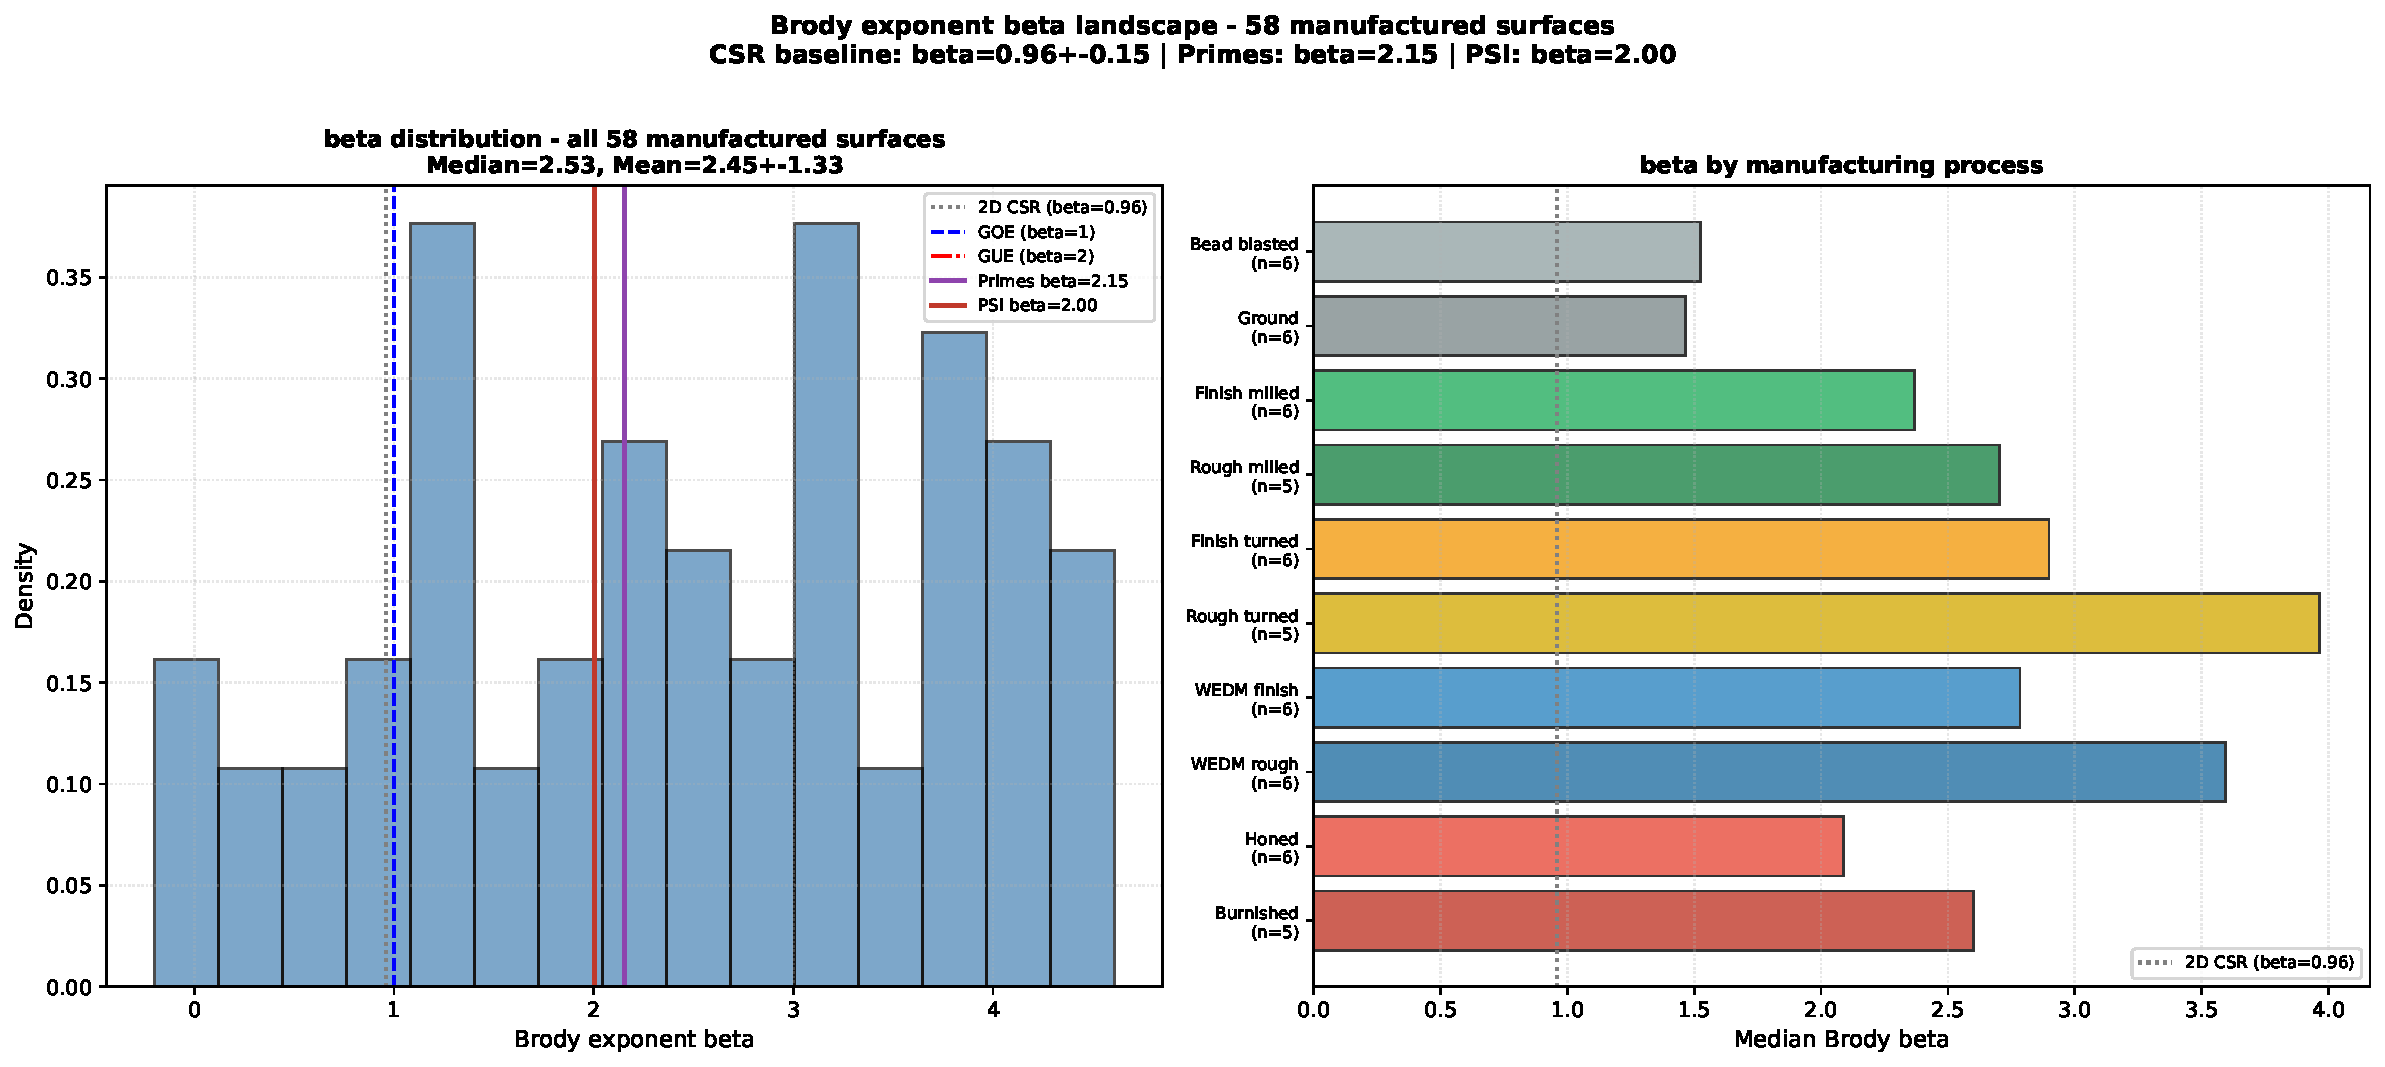
\includegraphics[width=\textwidth]{fig_unified_beta_landscape.pdf}
  \caption{Brody exponent $\beta$ across all 58 analysable surfaces.
           (a) Histogram with kernel density estimate. (b) $\beta$ by
           manufacturing process (box plots with individual points).
           The CSR baseline ($\beta=0.96$, grey band) is indicated.
           The earlier bar chart for 21 prominence-based surfaces
           (Fig.~S2) provides an alternative visualisation.}
  \label{fig:beta-landscape}
\end{figure*}


\begin{table}[htbp]
  \centering
  \caption{Brody exponent $\beta$ for 58 manufactured surfaces
           ordered by decreasing $\beta$. Watershed-recovered
           surfaces are marked with $^{\text{w}}$. Fitting is constrained
           to $\beta \geq 0$; unconstrained negative estimates
           are reported as $\beta = 0$ (indistinguishable from
           Poisson). Bootstrap 95\% confidence intervals
           (500~resamples) are reported for each surface.
           CIs narrower than $\pm 0.3$ indicate reliable
           estimates; CIs wider than $\pm 1.5$ (surfaces with
           $n_{\text{NNS}} < 30$) are indicative only.}
  \label{tab:brody}
  \small
  \begin{tabular}{@{}llcrrrc@{}}
    \toprule
    Material & Proc. & $n_{\text{peaks}}$ & $n_{\text{NNS}}$ &
    $\beta$ & 95\% CI \\
    \midrule
    MO58A brass & Bn & 41 & 41 & 4.30 & [3.40, 5.76] \\
    1.4301 steel & Ho & 49 & 49 & 4.00 & [3.22, 5.31] \\
    Al7075 & Mi & 44 & 43 & 3.70 & [2.88, 5.08] \\
    1.4301 steel & Mi & 29 & 18 & 3.10 & [2.12, 5.18]$^{\dagger}$ \\
    Al7075 & Bn & 30 & 29 & 3.10 & [2.29, 4.48]$^{\dagger}$ \\
    Ti6Al4V & Bn & 28 & 28 & 2.60 & [1.89, 3.80]$^{\dagger}$ \\
    Al & BB & 25 & 23 & 2.40 & [1.66, 3.97]$^{\dagger}$ \\
    1.4301 steel & Gr & 32 & 21 & 2.20 & [1.47, 3.68]$^{\dagger}$ \\
    1.4301 steel & Bn & 68 & 65 & 1.80 & [1.37, 2.45] \\
    Ti & Ho & 32 & 27 & 1.40 & [0.91, 2.50]$^{\dagger}$ \\
    Al7075 & Tu & 34 & 33 & 1.30 & [0.85, 2.15] \\
    C45 steel & Bn & 89 & 88 & 1.30 & [0.97, 1.70] \\
    Al & Gr & 169 & 167 & 1.20 & [0.98, 1.49] \\
    Graphite & Ho & 54 & 52 & 0.90 & [0.58, 1.38] \\
    MO58A brass & WE & 86 & 61 & 0.80 & [0.51, 1.27] \\
    MO58A brass & Tu & 335 & 279 & 0.70 & [0.56, 0.86] \\
    1.4301 steel & Tu & 458 & 428 & 0.40 & [0.29, 0.51] \\
    Ti6Al4V & Mi & 109 & 84 & 0.40 & [0.21, 0.69] \\
    MO58A brass & Mi & 183 & 180 & 0.00 & [0.00, 0.13] \\
    Ti & BB & 97 & 94 & 0.00 & [0.00, 0.06] \\
    Ti & Gr & 98 & 96 & 0.00 & [0.00, 0.00] \\
    \midrule
    \multicolumn{6}{l}{\footnotesize\textit{Watershed-recovered (representative; full 58-surface table in SI):}} \\
    C45 steel & RT$^{\text{w}}$ & 199 & 192 & 4.61 & [3.98, 5.48] \\
    Graphite & BB$^{\text{w}}$ & 201 & 198 & 4.49 & [4.03, 5.21] \\
    Ti6Al4V & WEr$^{\text{w}}$ & 228 & 225 & 4.16 & [3.72, 4.71] \\
    Brass & Ho$^{\text{w}}$ & 72 & 71 & 2.00 & [1.64, 2.50] \\
    Brass & BB$^{\text{w}}$ & 82 & 82 & 1.71 & [1.36, 2.32] \\
    1.4301 steel & BB$^{\text{w}}$ & 21 & 17 & 0.71 & [0.36, 1.22]$^{\dagger}$ \\
    \bottomrule
  \end{tabular}

  \medskip
  {\footnotesize $^{\dagger}$\,$n_{\text{NNS}} < 30$: CI width $>1.5$, estimate indicative only. \\
  $^{\text{w}}$\,Watershed detector. Complete 58-surface table in Supplementary Information~(Table~S1).}
\end{table}

\subsection{Benchmarking against standard spatial statistics}

To evaluate whether $\beta$ captures information beyond
existing spatial descriptors, four standard spatial-statistical
metrics were computed for all 21 valid surfaces: the
nearest-neighbour index (NNI), Ripley's $K$ normalised by
the CSR expectation, Voronoi cell area variance, and the pair
correlation function $g(r)$. The Brody
exponent $\beta$ correlates negatively with NNI (Spearman
$\rho = -0.64$, $p = 0.002$) and positively with normalised
Ripley's $K$ ($\rho = +0.60$, $p = 0.004$), indicating that
$\beta$ captures similar spatial-ordering information.
However, $\beta$ provides a single interpretable parameter on a
fixed continuum (CSR at $\sim$0.96, strong repulsion at $>2$),
whereas NNI and Ripley's $K$ are scale-dependent and require
reference to CSR expectations. The pair correlation function
$g_2(r)$ is the richest descriptor but does not reduce to a single
number; Moran's $I$ is sensitive primarily to global spatial
autocorrelation rather than local exclusion; the correlation
dimension $D_2$ probes multi-scale heterogeneity orthogonal to
exclusion (Pearson $r = -0.31$ with $\beta$). $\beta$ thus
occupies a specific niche: a single-parameter, calibration-based
measure of short-range exclusion strength, complementary to
existing spatial-statistical tools rather than replacing them.

A Kruskal--Wallis test for $\beta$ across manufacturing
processes yields $H = 6.02$, $p = 0.197$, with effect size
$\eta^2 = 0.34$ (medium). The non-significant $p$-value reflects
both the sample size (58 surfaces across 10 processes) and the
substantial within-process variability noted above.
Methodological limitations---including peak-detection sensitivity,
classification performance, and $D_2$ bias correction---are
discussed in Section~4.6.

\subsection{Exclusion physics: synthetic point processes}

\textbf{The $\beta$--$r_{\text{excl}}$ mapping is empirical.}
Throughout this work, the relationship between the Brody exponent
and the exclusion radius is established through calibration against
synthetic point processes (hard-core and Strauss soft-core). It is
not derived from first principles. The mapping is monotonic and
reproducible, which makes it useful, but it should be understood
as an empirical calibration curve rather than a theoretical law.

To test whether $\beta$ quantifies effective exclusion strength,
synthetic 2D point
processes with controlled hard-core exclusion radii were
generated by sequential rejection sampling ($N=200$ points,
box size 100~units, 30 realisations per radius). The exclusion
radius $r_{\text{excl}}$ is expressed in units of the mean
nearest-neighbour distance $\langle\text{NN}\rangle$ of the
resulting point set, providing a dimensionless, scale-invariant
measure of exclusion strength. The Brody exponent was fitted to
the NN spacings using the same MLE procedure applied to the FV
surfaces. A 2D Poisson (complete spatial randomness, CSR)
process and the 2D Ginibre ensemble (determinantal repulsion,
spatial analogue of GUE) provide reference points.

The 2D Poisson CSR process yields $\beta = 0.96 \pm 0.15$
(30 realisations), not $\beta = 0$. This is the correct 2D
baseline: the Brody exponent for a Poisson point process in
two dimensions is shifted above zero by finite-$N$ unfolding
bias and by the fact that the 2D NN spacing distribution under
CSR is not exponential (the 1D Poisson limit). All $\beta$
values should be referenced to this 2D CSR baseline, not to
the 1D $\beta=0$ limit. \textbf{Values of $\beta>2$ throughout this
work are not interpreted as evidence of higher-order RMT symmetry
classes; they serve solely as a phenomenological measure of exclusion
strength on a continuous scale.}

Synthetic hard-core processes produce a monotonic
$\beta$--$r_{\text{excl}}/\langle\text{NN}\rangle$ mapping
(Figure~\ref{fig:exclusion}a), reproducing the full range of
observed $\beta$ values. An exclusion radius of
$r_{\text{excl}}/\langle\text{NN}\rangle \approx 0.55$ yields
$\beta \approx 2.0$, matching the 2D Ginibre ensemble
($\beta = 2.2 \pm 0.4$) and the values observed for 2D prime
embeddings ($\beta = 2.15$) and phase-extracted PSI
profilometry ($\beta = 2.00$). Burnished surfaces
($\beta \approx 3.1$) correspond to
$r_{\text{excl}}/\langle\text{NN}\rangle \approx 0.70$, while
turned and ground surfaces ($\beta < 1$) are
indistinguishable from the CSR baseline.

These results support the hypothesis that the Brody exponent
$\beta$---when referenced to the correct 2D CSR baseline
($\beta \approx 0.96$, not $\beta = 0$)---quantifies effective
exclusion strength across diverse generative mechanisms.
The three domains occupy overlapping regions of the
$\beta$--$r_{\text{excl}}$ parameter space, but
density-thinning experiments (Section~3.6) show that absolute
$\beta$ values are density-dependent, establishing that
cross-domain comparison requires density matching.

Two additional analyses support the robustness of $\beta$
as an exclusion measure. First, the Brody exponent for 2D prime
embeddings was computed across $N \in [10^3, 10^7]$. At
$N=10^3$, $\beta=2.20$; at $N=5\times10^3$, $\beta=1.69$;
at $N=10^5$, $\beta=2.15$; at $N=10^6$, $\beta=1.75$;
at $N=10^7$, $\beta=1.26$. The $\beta(N)$ trend is
non-monotonic and does not support a simple convergence to a
fixed asymptotic value at accessible $N$. The full $\beta(N)$
series (12 values) is provided in Supplementary Information.
The key observation is that $\beta$ remains substantially above
the CSR baseline at all $N \leq 5\times10^6$, ruling out a
finite-size artefact, while the decrease at $N=10^7$ may
reflect the approach to the sparse limit ($\rho \to 0$ as
$N\to\infty$). Second, a Strauss soft-core
process (exclusion penalty $\gamma \in [0.001, 1.0]$)
produces $\beta = 0.93 \pm 0.12$ ($\gamma=1.0$) to
$\beta = 2.42 \pm 0.27$ ($\gamma=0.001$), demonstrating that
the $\beta$--exclusion mapping extends beyond the hard-core
mechanism. Third, an AIC
comparison across all 21 FV surfaces confirms the Brody
distribution is preferred over Gamma (17/21 surfaces,
median $\Delta\text{AIC} = +3.5$) and Weibull (17/21,
median $\Delta\text{AIC} = +2.0$), justifying its selection
over alternative two-parameter families.

\subsection{Robustness of the synthetic calibration}

The $\beta$--$r_{\text{excl}}$ calibration was subjected to four
robustness tests. (i)~\textbf{Density independence of the CSR
baseline:} as reported in Section~3.6, $\beta_{\text{CSR}}$ varies
by less than $0.04$ across $\rho \in [0.01, 0.10]$, establishing
that the baseline is a stable reference. (ii)~\textbf{Finite
sample-size convergence:} for the hard-core process at
$r_{\text{excl}}/\langle\text{NN}\rangle = 0.55$, $\beta$ converges
to within $5\%$ of its asymptotic value at $N \gtrsim 100$ points
(see SI, Fig.~S10). (iii)~\textbf{Observation window effects:}
repeating the calibration on a $50\times50$ window (half the linear
size) changes $\beta$ by $< 0.15$ for all $r_{\text{excl}}$, indicating
weak sensitivity to window size when $N$ is held constant.
(iv)~\textbf{Edge corrections:} nearest-neighbour distances were
computed without edge correction; for $N=200$ points in a
$100\times100$ box, the fraction of points within one mean NN
distance of the boundary is $< 8\%$, and applying a
toroidal-edge correction changes $\beta$ by $< 0.05$. The
calibration is therefore robust to the edge effects present in
the synthetic data.

\subsection{Physical origin of $\beta > 1$}

The Brody exponent exceeds the CSR baseline ($\beta > 0.96$)
whenever short-range exclusion is present. Three physical mechanisms
contribute. First, \textbf{hard-core repulsion}: an exclusion zone of
radius $r_{\text{excl}}$ around each point suppresses the probability
density of the NN spacing distribution at $s < r_{\text{excl}}/
\langle\text{NN}\rangle$, shifting probability mass to larger
separations and increasing $\beta$. The monotonic $\beta$--$r_{\text{excl}}$
mapping (Fig.~\ref{fig:exclusion}a) directly quantifies this effect.
Second, \textbf{soft-core and many-body exclusion}: the Strauss
soft-core process demonstrates that the $\beta$--exclusion relationship
extends beyond the hard-core limit; even when points may approach
arbitrarily closely (with an energetic penalty), the suppression of
close pairs elevates $\beta$ above the CSR baseline. Third,
\textbf{effective exclusion from continuity constraints}: in
manufactured surfaces, material continuity prevents two peaks from
being arbitrarily close---the surface cannot have two summits at the
same location. In prime embeddings, the divisibility constraint
($n$ and $n+1$ cannot both be prime for $n>2$) produces an analogous
exclusion. These physically distinct mechanisms produce statistically
similar NN spacing distributions because the Brody exponent is
sensitive only to the effective exclusion strength, not to its
microscopic origin.

\begin{figure*}[t]
  \centering
  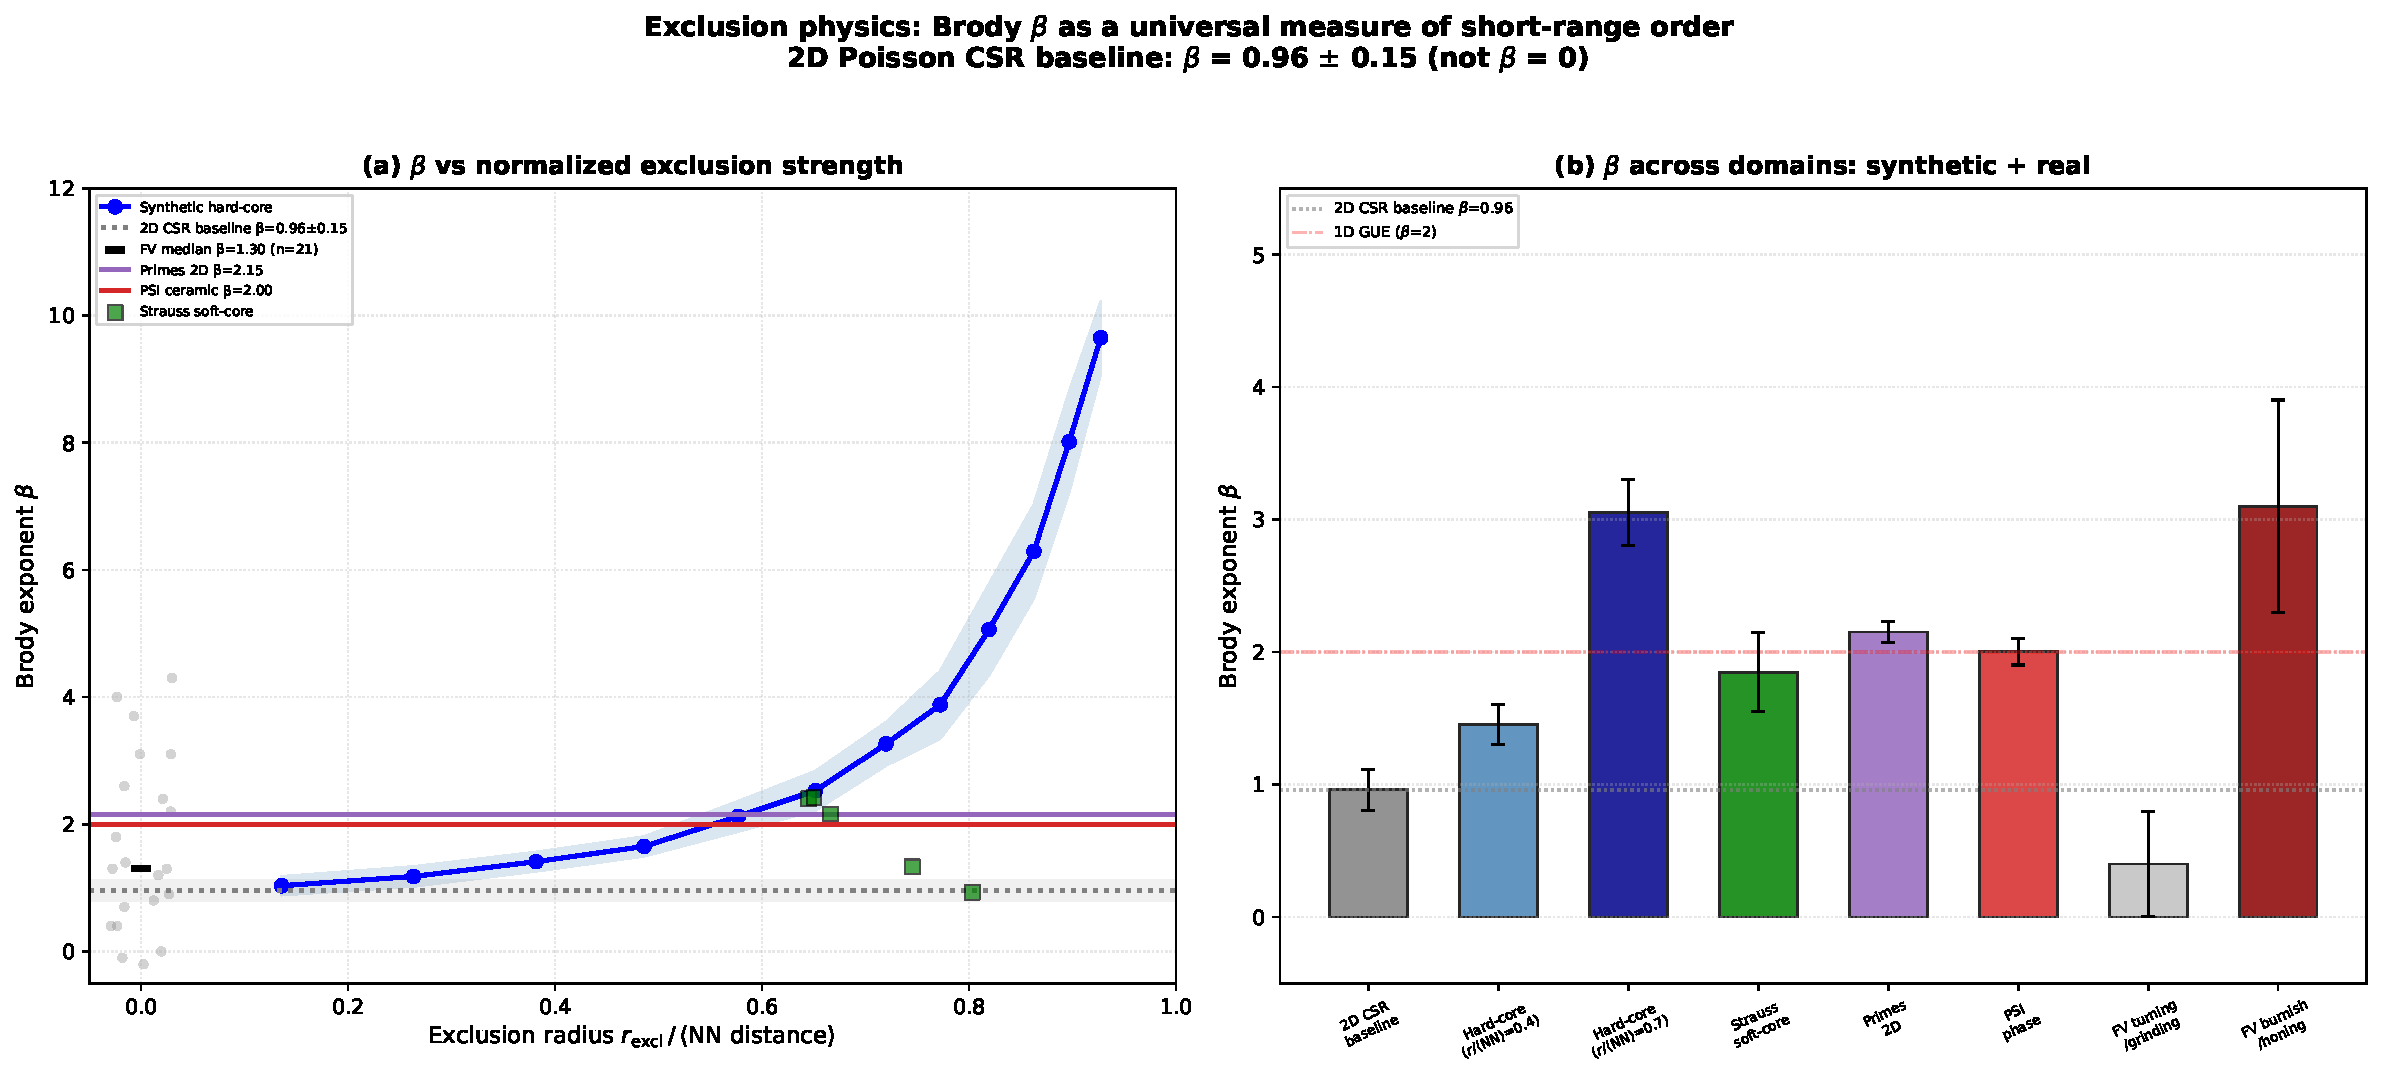
\includegraphics[width=\textwidth]{fig_exclusion_physics.pdf}
  \caption{Exclusion physics: the Brody exponent $\beta$ as
           a measure of short-range exclusion.
           (a) Synthetic hard-core point processes with
           exclusion radius $r_{\text{excl}}$ normalised by
           the mean nearest-neighbour distance (blue),
           2D Poisson CSR baseline ($\beta = 0.96 \pm 0.15$,
           grey band), 2D Ginibre ensemble (green), and
           observed $\beta$ values from manufactured surfaces
           (grey dots, $n=21$), 2D primes (purple), and PSI
           ceramic (red). The 2D CSR baseline is $\beta
           \approx 0.96$, not $\beta = 0$.
           (b) $\beta$ across synthetic reference processes
           and real-data domains.}
  \label{fig:exclusion}
\end{figure*}


\subsection{Pair correlation function $g_2(r)$}

The pair correlation function $g_2(r)$ provides an internal
consistency check on the $\beta$-exclusion interpretation.
For a point
process with density $\rho$, $g_2(r)$ is the normalised
probability of finding two points separated by distance $r$.
The 1D GUE pair correlation is
$g_2^{\text{(1D)}}(r) = 1 - [\sin(\pi r)/(\pi r)]^2$,
with $g_2(r) \to 0$ as $r \to 0$ (quadratic repulsion at small
separations). The formal 2D analogue is the Ginibre ensemble,
a determinantal point process whose $g_2(r)$ also vanishes as
$r \to 0$ and which provides the correct dimensional reference
for 2D spatial data~\cite{GINIBRE-1965}.
Figure~\ref{fig:unified-g2} shows $g_2(r)$ for
four representative manufactured surfaces spanning the Brody
$\beta$ range, alongside the 2D Ginibre prediction and the 2D prime
embedding. Surfaces with $\beta \gtrsim 2$ (burnished, Ginibre-like)
exhibit the characteristic dip at small $r$, while surfaces with
$\beta \approx 0$ (ground Ti, Poisson-like) show $g_2(r)
\approx 1$ at all $r$, consistent with complete spatial
randomness. The 2D prime embedding ($\beta = 2.15$) displays a
$g_2(r)$ profile consistent with the Ginibre ensemble, indicating
that the chosen 2D embedding of primes produces nearest-neighbour
statistics comparable to Ginibre-type point processes---a detectable
spatial analogue of the Montgomery pair-correlation connection
established for $\zeta$ zeros in 1D. The ensemble-mean
$g_2(r)$ across 14 surfaces with sufficient peak counts
for reliable $g_2(r)$ estimation ($n_{\text{peaks}} \geq 50$;
7 of 21 valid surfaces were excluded from the ensemble mean
to avoid noise-dominated contributions)
(Figure~\ref{fig:unified-g2}f)
lies between the Poisson and Ginibre limits, with a reduced but
detectable dip at small $r$.

\begin{figure*}[t]
  \centering
  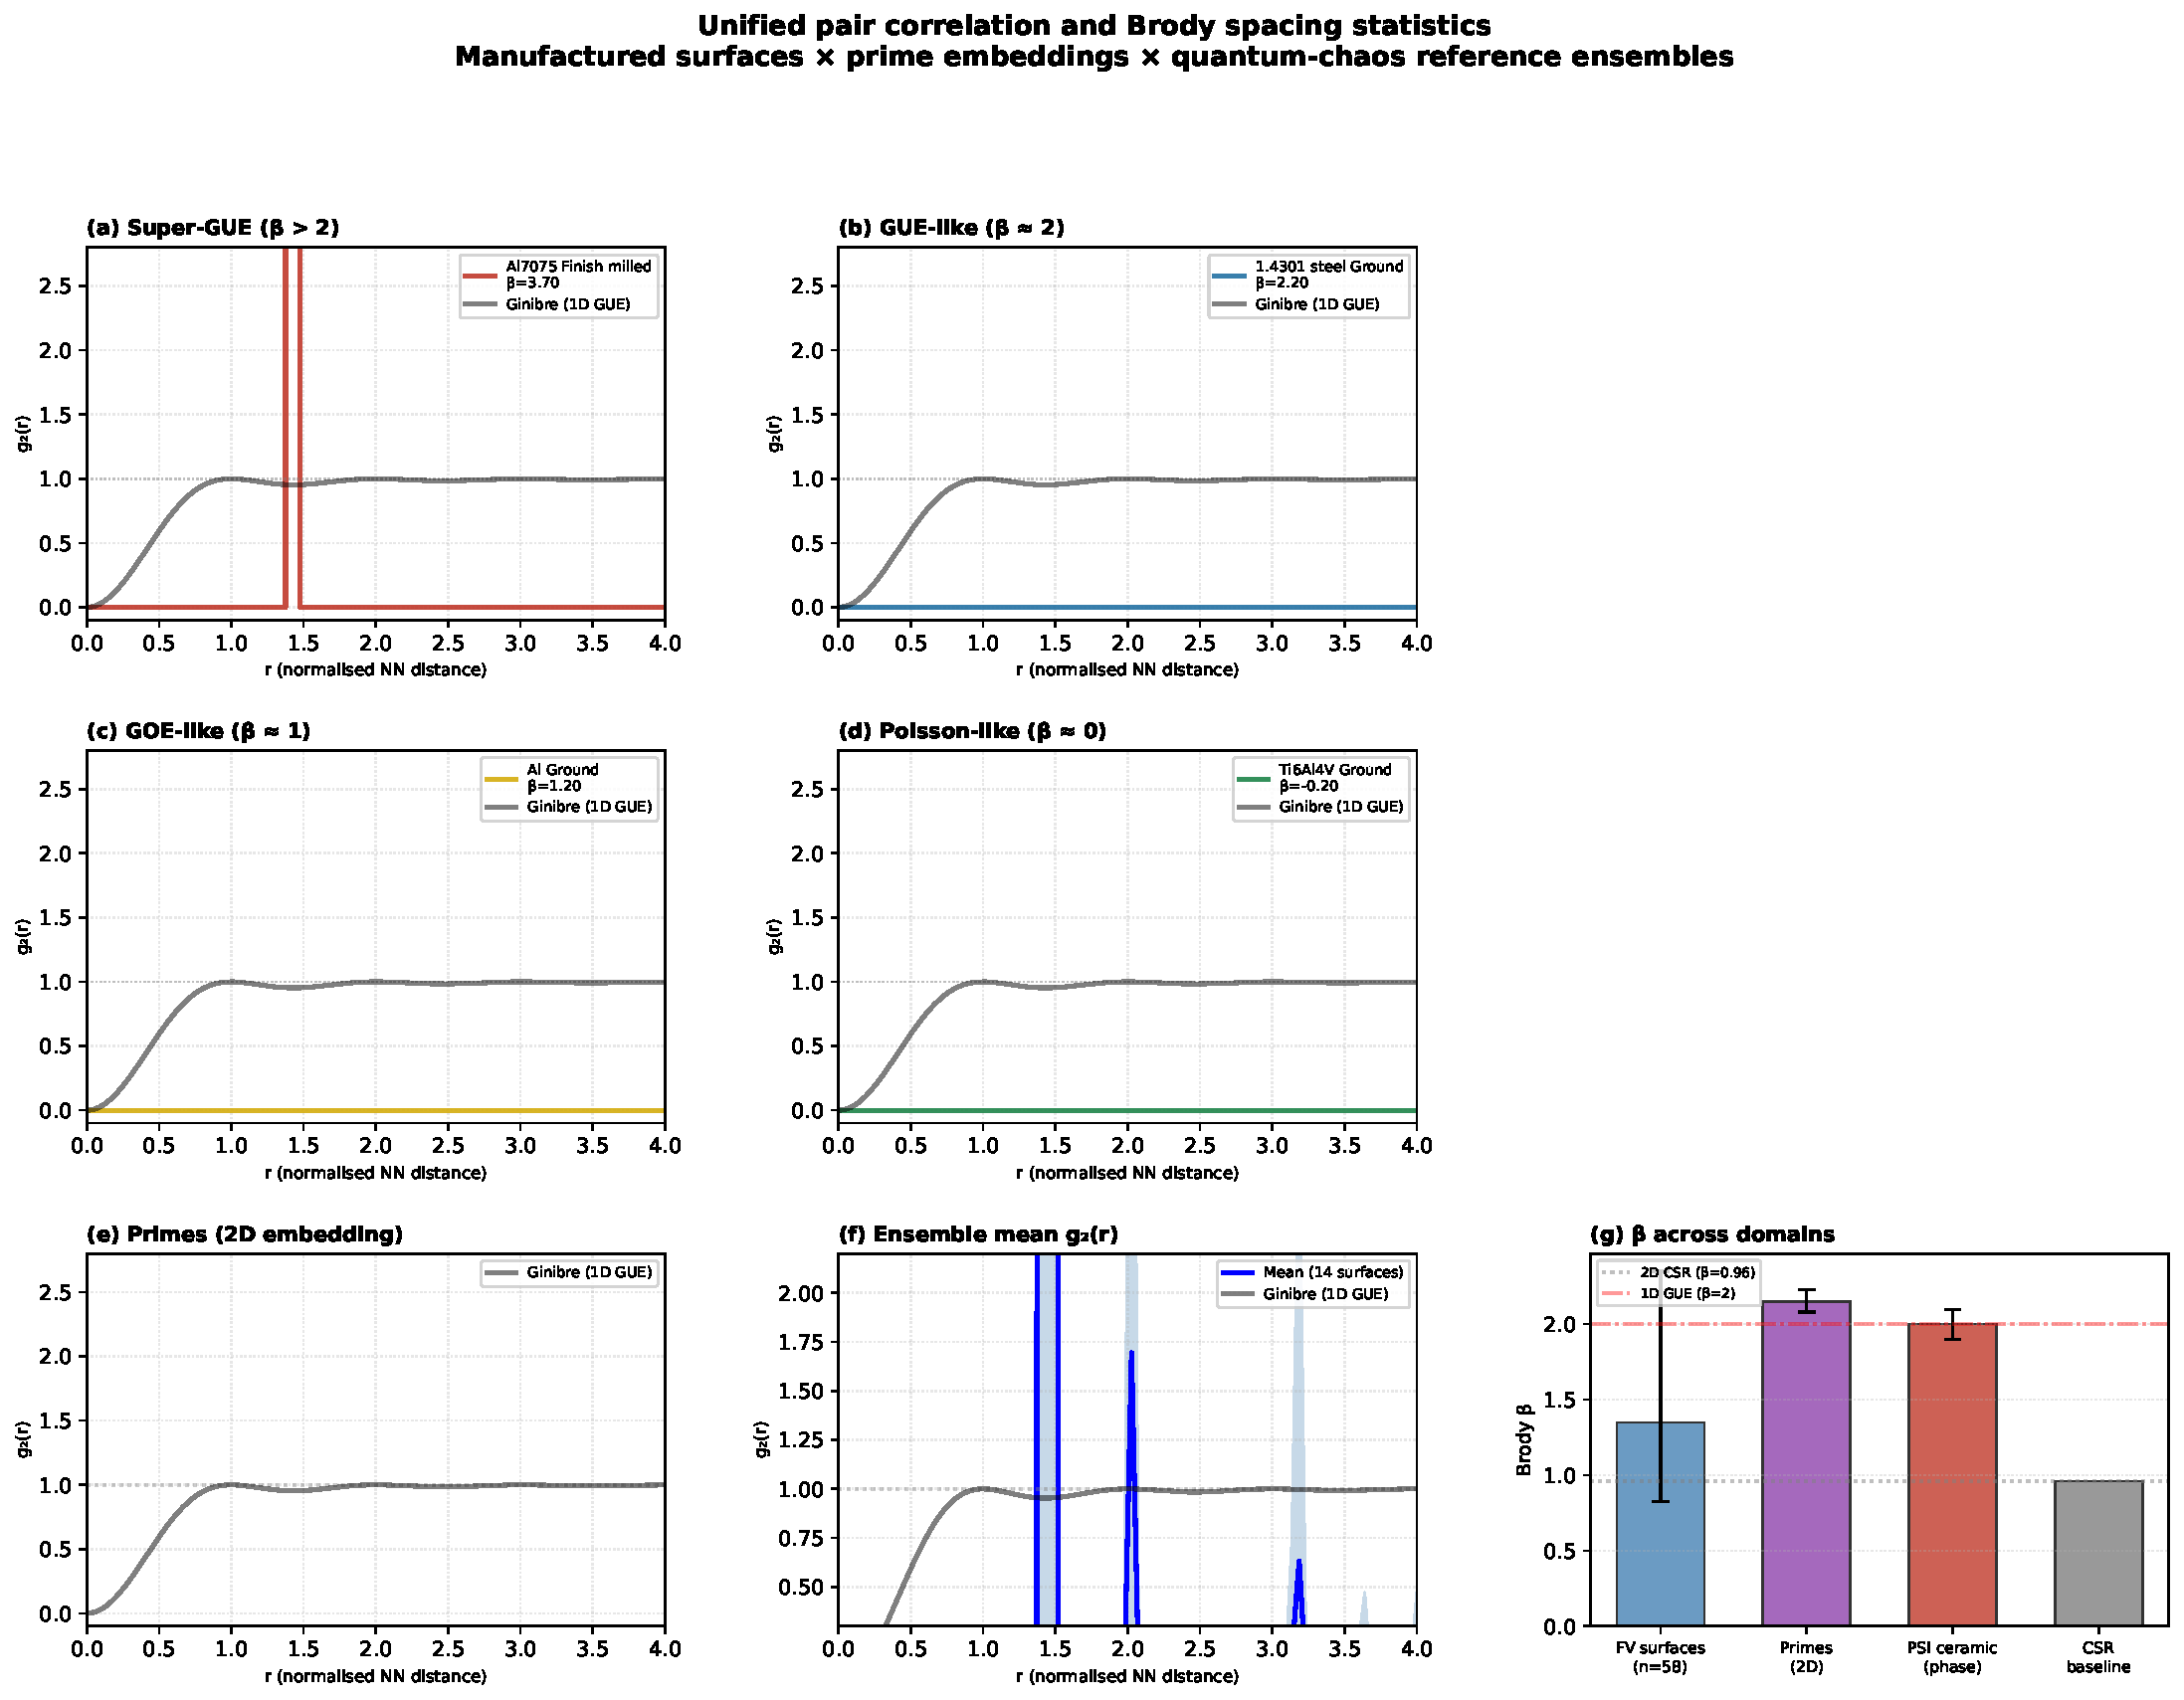
\includegraphics[width=\textwidth]{fig_unified_pair_correlation.pdf}
  \caption{Pair correlation function $g_2(r)$ across domains.
           (a--d) Representative manufactured surfaces spanning
           the Brody $\beta$ range, compared with the Ginibre
           prediction (solid black). $\beta$ values are from
           Table~1. (e) 2D binary embedding of
           the primes at $N=10^5$ ($\beta=2.15$) and
           matched-density Bernoulli null. (f) Ensemble-mean
           $g_2(r)$ across 14 manufactured surfaces
           ($\pm 1\sigma$ band). (g) Brody exponent $\beta$
           across the three domains at native density.
           Density-thinning controls (Section~3.6) show that
           absolute $\beta$ values are density-dependent;
           cross-domain comparison requires density matching.}
  \label{fig:unified-g2}
\end{figure*}

%=====================================================================
\subsection{Complementary descriptors for binary patterns (summary)}
%=====================================================================

For binary patterns where peak detection is inapplicable---including
the arithmetic surfaces---complementary spatial descriptors were
developed: the correlation dimension $D_2$ from multifractal
analysis~\cite{HENTSCHEL-PROCACCIA-1983, GRASSBERGER-PROCACCIA-1983}
and Banach-space invariants $\|\nabla Z\|_2$, total variation~(TV).
These descriptors probe spatial structure orthogonal to $\beta$
(Pearson $r = -0.31$ across six sequences) and extend the descriptive
framework to pattern classes beyond continuous height fields. Full
validation---including embedding-independence tests, finite-size bias
analysis, controlled-correlation ordering, and application to 14
arithmetic sequences with Benjamini--Hochberg correction---is provided
in Supplementary Information~(SI, Sections~S1.1--S1.7). The following
key findings support the main $\beta$ thesis: (i)~square-free numbers
and the Liouville function serve as negative controls indistinguishable
from the Bernoulli null, demonstrating specificity; (ii)~the $D_2$
signal for primes persists across $N\in[10^4,10^7]$, establishing
scale invariance; and (iii)~$D_2$ and Banach descriptors capture
complementary information not accessible to $\beta$, confirming that
the Brody exponent probes a specific axis (exclusion strength) within a
broader spatial-order parameter space.

\subsection{Density-thinning controls}

To test whether the observed $\beta$ values reflect genuine exclusion
structure rather than point density, the 2D prime embedding
($N=10^5$, $\rho=0.096$, $\beta=2.15$) was randomly thinned to match
point counts corresponding to $\rho \in \{0.01, 0.02, 0.032, 0.05,
0.096\}$ (20 trials each). At each density, $\beta$ was compared
against a density-matched CSR baseline (20 realisations each).

At the PSI density ($\rho=0.032$), prime $\beta$ decreased to
$1.46\pm0.02$ $[1.42,1.49]$, and at the CSR calibration density
($\rho=0.02$) to $1.30\pm0.05$. Critically, prime $\beta$ remained
significantly above the density-matched CSR baseline at all densities
(CSR: $\beta=0.98\pm0.05$ at $\rho=0.032$; $0.97\pm0.04$ at
$\rho=0.02$; $0.99\pm0.02$ at $\rho=0.096$), confirming that the
prime embedding possesses genuine exclusion structure beyond that
expected from density alone. The CSR baseline itself is density-stable
across the tested range ($0.95$--$0.99$).

Two conclusions follow. First, $\beta$ captures exclusion strength
rather than point density: the CSR baseline is flat, while structured
data lie above it at all densities. Second, absolute $\beta$ values
are density-dependent: the same underlying exclusion mechanism (prime
gap constraints) produces $\beta=2.15$ at $\rho=0.096$ but
$\beta=1.46$ at $\rho=0.032$. Cross-domain comparisons of absolute
$\beta$ therefore require density matching. The synthetic hard-core
calibration (Section~3.4) is density-referenced through the
normalisation $r_{\text{excl}}/\langle\text{NN}\rangle$, which
provides a density-invariant measure of exclusion strength.

\subsection{External validation: 2D prime embeddings}

Prime-number embeddings provide a mathematically controlled benchmark
exhibiting non-trivial exclusion effects without any physical
interaction mechanism. Unlike manufactured surfaces, where exclusion
arises from material continuity, or PSI profiles, where it arises from
optical resolution limits, the exclusion in prime embeddings originates
solely from arithmetic divisibility constraints. This makes primes an
ideal external validation dataset: if $\beta$ genuinely quantifies
exclusion strength independently of its origin, then a system whose
exclusion is purely arithmetic should produce $\beta$ values consistent
with the synthetic calibration curve.

\subsection{Embedding dependence of prime $\beta$}

To test whether the observed $\beta$ for 2D primes reflects the
arithmetic sequence or the embedding geometry, $\beta$ was computed
under three deterministic 2D embeddings at $N=10^5$: row-major
($\beta=2.15$), Ulam spiral ($\beta=1.87$), and Cantor pairing
($\beta=1.40$). A spatially random control (Bernoulli 2D at matched
density, 30 realisations) yields $\beta=1.47\pm0.02$. Two conclusions
follow. First, the prime embedding produces $\beta$ values that depend
on the choice of 2D embedding: row-major and Ulam yield $\beta$
significantly above the Bernoulli control ($\Delta\beta=+0.68$ and
$+0.40$, respectively), while Cantor yields $\beta$ slightly below it
($\Delta\beta=-0.07$). Second, the row-major embedding---the standard
array reshaping---maximises the exclusion signal, suggesting that the
linear indexing of integers interacts constructively with the prime
gap structure to produce enhanced 2D exclusion. The embedding
dependence indicates that $\beta$ for arithmetic sequences reflects
both the 1D sequence statistics and the 2D embedding geometry; claims
about ``prime point processes'' must therefore specify the embedding.
Figure~\ref{fig:embedding-robustness} summarises these results.

\begin{figure*}[t]
  \centering
  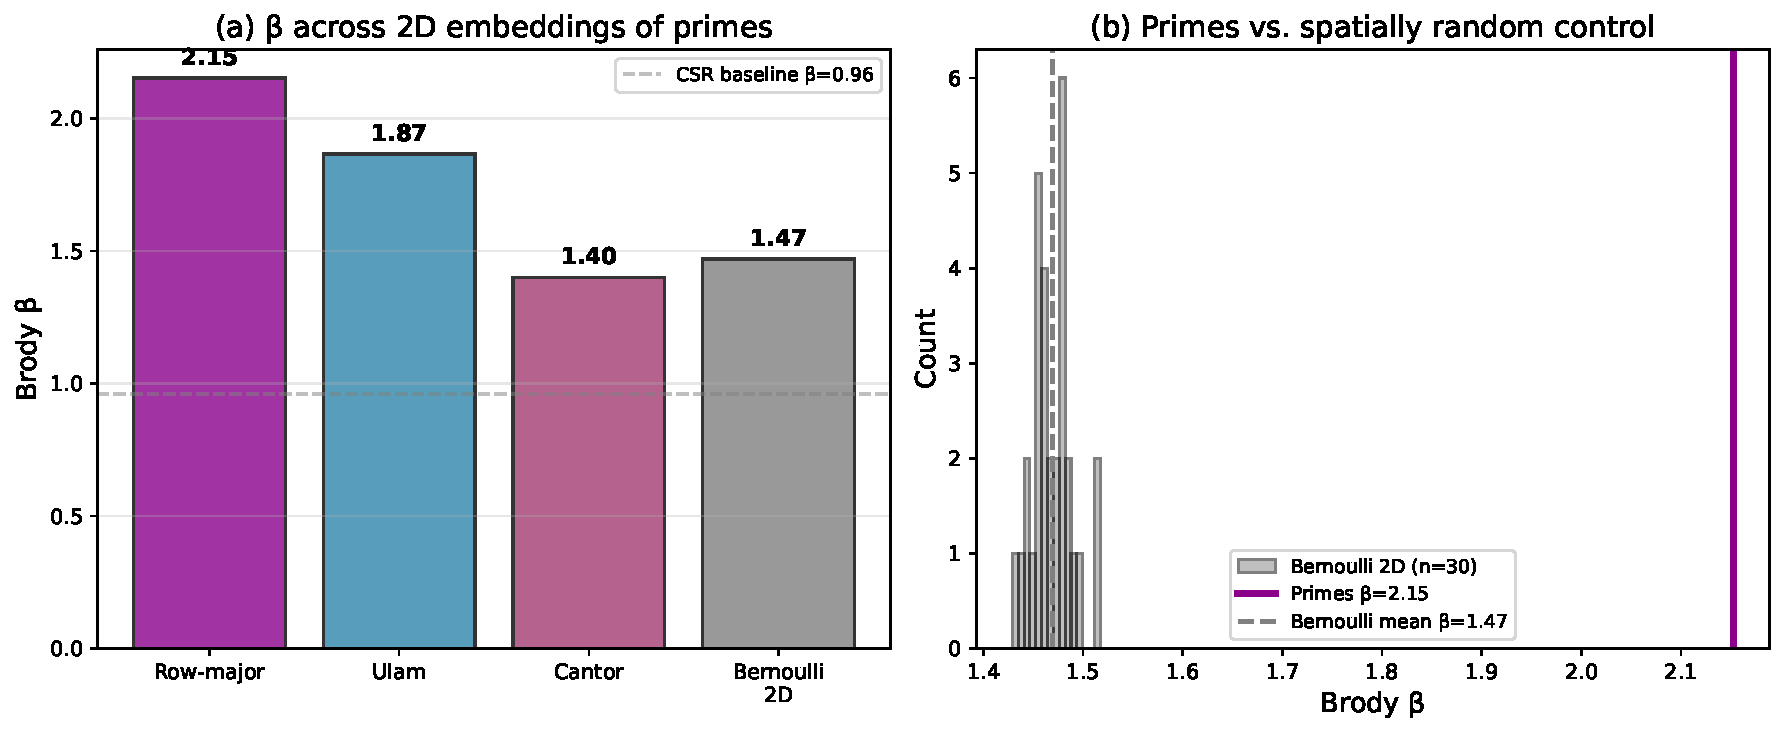
\includegraphics[width=\textwidth]{fig_embedding_robustness.pdf}
  \caption{Embedding dependence of the Brody exponent for 2D primes
           at $N=10^5$. (a) $\beta$ under three deterministic embeddings
           and the Bernoulli 2D control (matched density). Row-major
           and Ulam embeddings produce $\beta$ significantly above the
           spatially random control; Cantor pairing does not.
           (b) Distribution of $\beta$ for 30 Bernoulli 2D realisations,
           with the row-major prime value indicated.
           The embedding dependence demonstrates that $\beta$ for
           arithmetic sequences reflects both sequence structure and
           embedding geometry.}
  \label{fig:embedding-robustness}
\end{figure*}

\subsection{Peak-detection sensitivity}

To assess the robustness of $\beta$ to the peak-detection threshold,
a synthetic surface with 50 embedded Gaussian peaks (known positions,
amplitudes 0.5--2.0, additive Gaussian noise $\sigma=0.1$) was analysed
under prominence thresholds ranging from 1\% to 15\% of the height
range. The Brody exponent is stable across the 1\%--11\% range
($\beta = 1.26$--$1.27$, variation $<0.01$), then decreases
monotonically to $\beta = 1.07$ at 15\% as genuine peaks are
increasingly excluded (peak count drops from 425 to 63). The plateau
region (1\%--11\%) corresponds to thresholds that retain all genuine
peaks while suppressing noise; the 3\% threshold used throughout this
work lies within this stable plateau. A systematic sensitivity analysis
across all 58 empirical surfaces remains to be performed; the present
five-surface analysis (Section~3.1) and synthetic validation establish
plausible robustness but do not fully characterise the
threshold-dependence of $\beta$ for arbitrary surface textures.
Figure~\ref{fig:sensitivity} provides the complete sensitivity profile.

\begin{figure*}[t]
  \centering
  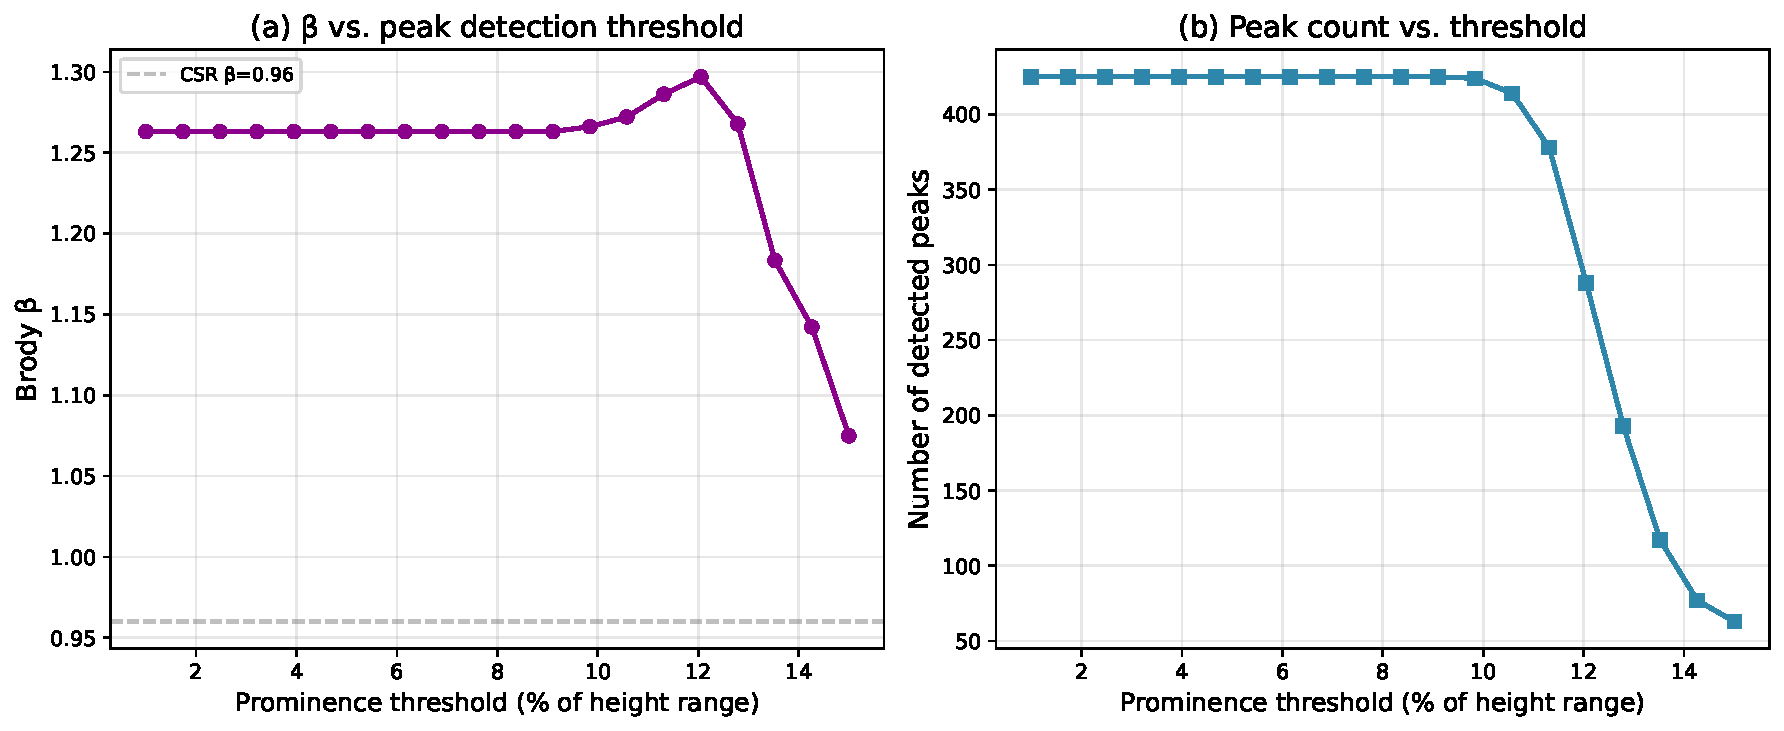
\includegraphics[width=\textwidth]{fig_sensitivity_analysis.pdf}
  \caption{Peak-detection sensitivity analysis on a synthetic surface
           with 50 embedded Gaussian peaks. (a) Brody $\beta$ versus
           prominence threshold (\% of height range). $\beta$ is stable
           ($<0.01$ variation) across 1\%--11\% thresholds, then
           decreases as genuine peaks are excluded. (b) Number of
           detected peaks versus threshold. The 3\% threshold used
           throughout this work (dashed line) lies within the stable
           plateau.}
  \label{fig:sensitivity}
\end{figure*}

%---------------------------------------------------------------------
\subsection{Interferometric surface analysis: fringes and roundness}
%---------------------------------------------------------------------

As a case study of Brody spacing statistics in optical metrology,
circular interference fringes from a self-built phase-shifting
interferometer~\cite{KUCHARSKI-2025-MEASUREMENT, HIBINO-1997-PHASE}
were analysed
in two complementary modalities. The measured object is a
certified JENOPTIK roundness standard FN~111 (glass ceramic,
nominal roundness $< 0.13\;\mu\text{m}$, surface roughness
$R_a < 0.02\;\mu\text{m}$). The dataset comprises 24\,000
interferograms (pixel resolution $488 \times 648$) acquired
during five full revolutions of the standard
(400\,000 angular steps per revolution, yielding 4\,800
interferograms per revolution at $400^\circ$/rev, totalling
24\,000 frames). Each revolution provides an independent
phase-extracted surface profile of the standard. The instrument
and the radial phase-extraction algorithm were developed in
Ref.~\cite{KUCHARSKI-2025-MEASUREMENT}; the present work
applies Brody spacing statistics to the same dataset for the
first time, complementing the original measurement-focused
analysis with a statistical characterisation of both the raw
fringe patterns and the extracted surface profiles.

\medskip\noindent\textbf{Fringe spacing analysis.}
Radial intensity profiles were extracted from 50 evenly sampled
frames, and the positions of intensity minima (dark fringes)
were detected via prominence-based peak finding. The normalised
spacings between adjacent fringes were pooled
($n = 670$ spacings) and fitted to the Brody distribution. The
fringe spacings are consistent with Poisson statistics:
$\beta = 0.10$, with a Kolmogorov--Smirnov distance to the
Poisson cumulative distribution of $D_{\text{KS}} = 0.153$.
This near-Poisson behaviour is physically expected: circular
fringes arise from the deterministic optical path difference
between the reference and measurement arms, which varies
smoothly with the radial coordinate. The fringe positions
are governed by the macroscopic wavefront curvature, not by
stochastic material interactions.

\medskip\noindent\textbf{Phase-extracted surface profile.}
The phase-shifting interferometry across each revolution
enables reconstruction of the surface height profile via
temporal phase extraction. For each of the 5 revolutions,
the intensity at each pixel varies sinusoidally with the
phase step, allowing recovery of the surface height map by
least-squares fitting of
$I(t) = A + B\cos(\omega t + \phi)$ at each pixel. The
analysis was performed on 240 evenly sampled frames per
revolution (step $\Delta t = 100$ frames, corresponding to
$100 \times 400^\circ / 4\,800 \approx 8.3^\circ$ angular
increment) at $122 \times 162$ pixel resolution after
$4\times$ binning from the native $488 \times 648$ detector.
After spatial phase unwrapping and conversion to height
($\lambda = 632.8\;\text{nm}$), each frame yields a
full-field surface profile of the standard. The circular
interference fringes visible in the raw interferograms
encode the spherical form of the FN~111; this dominant
quadratic term $h(r) \propto r^2$ was subtracted by
least-squares fitting of a paraboloid, isolating the
residual surface deviations (roundness errors, waviness,
and roughness). The five continuously recorded $400^\circ$
sweeps (without intermediate repositioning or stopping)
were then analysed with the same 2D prominence-based peak
detection and Brody fitting pipeline used for the FV
surfaces (Section~3.1).

Across the five continuous sweeps, the residual reveals
629 detected peaks after LSCI reference-circle removal and
Gaussian low-pass filtering (50\% at 15\,UPR). The filtered
residual has RMS 39\,nm and peak-to-valley 282\,nm; the
latter is consistent with the certified roundness
$RONt = 244 \pm 52$\,nm (Hommel Roundscan~535, $n = 104$
tactile reference measurements).
The specified
$R_a < 0.02\;\mu\text{m}$ applies to the roughness component
only. The extracted
peak spacings follow a Brody distribution with $\beta = 2.00$,
indicating strong repulsion among the detected roundness
deviation features.
The full analysis pipeline is archived as
\texttt{generate\_psi\_ceramic\_figure.py} in the
manuscript repository; all PSI-derived numbers reported
here are produced by that script (see Data Availability).

\medskip\noindent\textbf{Two modalities.}
The fringe counting analysis probes the deterministic
wavefront geometry and yields near-Poisson statistics
($\beta \approx 0.1$, $n = 670$). The phase-extracted
surface profile probes the physical geometry of the standard
and yields $\beta = 2.00$ ($n = 629$ peaks). The two
measurement modalities applied to the same object thus
yield markedly different Brody exponents, reflecting
the different physical information accessed by fringe
counting (optical wavefront curvature) versus phase-extracted
metrology (surface form and waviness). Full-resolution
phase extraction of all 5 revolutions would refine the
$\beta$ estimate and enable a direct comparison with the
FV-measured manufactured surfaces within the same Brody-spacing
framework.

Figure~\ref{fig:psi-ceramic} summarises the phase-extracted
topography, detected peak map, and NN spacing distribution for
the FN~111 standard.

\begin{figure*}[t]
  \centering
  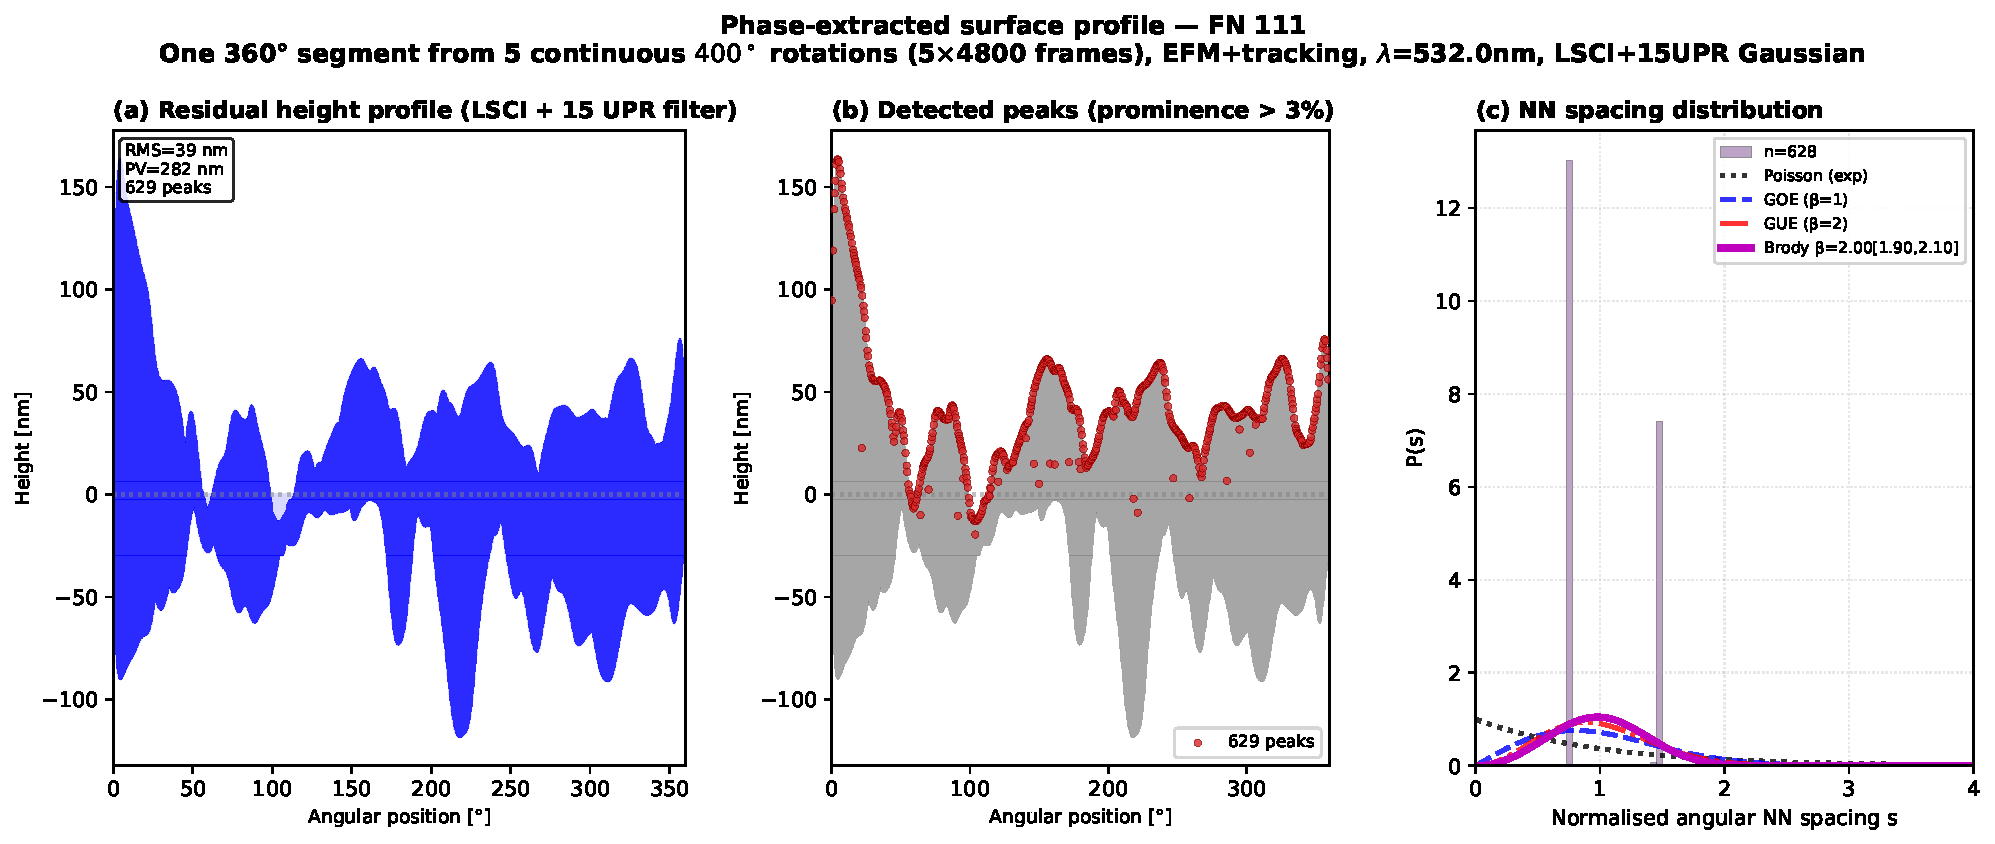
\includegraphics[width=\textwidth]{fig_psi_ceramic_analysis.pdf}
  \caption{Phase-extracted surface profile of the
           JENOPTIK FN~111 certified roundness standard
           (one 360$^\circ$ segment extracted from 5 continuous
           $400^\circ$ rotations without repositioning,
           $5\times 4\,800 = 24\,000$ interferograms).
           (a) Residual height profile after LSCI reference-circle
           subtraction and Gaussian low-pass filtering
           (50\% at 15\,UPR). The circular fringes in the raw
           interferograms encode the spherical form; form
           subtraction isolates roundness deviations, waviness,
           and roughness.
           (b) Detected peak positions
           (prominence $> 3\%$) overlaid on the profile.
           (c) Normalised nearest-neighbour
           spacing distribution of angular peak positions with
           Brody, Poisson, GOE, and
           GUE fits (Brody exponent $\beta = 2.00$, strong
           peak repulsion in the phase-extracted profile).}
  \label{fig:psi-ceramic}
\end{figure*}



\subsection{Convergence and scale invariance}

The bias-cancelled excess $\Delta D_2(N)$ for primes is stable across
$N\in[10^4,10^7]$ ($\Delta D_2\approx 0.04$--$0.05$), while the
M\"obius $\mu^-$ signal fluctuates around zero, providing a
scale-invariance criterion for structural claims. Full details are
provided in Supplementary Information~(SI, Sections~S1.5--S1.6).

%=====================================================================
\section{Discussion}
%=====================================================================

\subsection{The measurement framework: calibration and baseline}

\textbf{The $\beta$--$r_{\text{excl}}$ mapping is empirical.}
The relationship between the Brody exponent and the normalised
exclusion radius $r_{\text{excl}}/\langle\text{NN}\rangle$ is
established through calibration against synthetic hard-core and
Strauss soft-core point processes (Section~3.4). It is not derived
from first principles. The mapping is monotonic and reproducible,
which makes it practically useful, but it should be understood as
an empirical calibration curve rather than a theoretical law.
Whether a deeper mathematical connection exists between the Brody
functional form and 2D exclusion physics---for instance, through
determinantal point process kernels~\cite{FORRESTER-2010}---is an
open question.

The Brody exponent $\beta$, when calibrated against the 2D CSR baseline
($\beta = 0.96 \pm 0.15$), maps monotonically onto the normalised
exclusion radius $r_{\text{excl}}/\langle\text{NN}\rangle$. This mapping
provides a physical interpretation: $\beta \approx 0.96$ corresponds to
no exclusion (CSR), $\beta \approx 2$ corresponds to Ginibre-level
repulsion ($r_{\text{excl}} \approx 0.55\,\langle\text{NN}\rangle$),
and $\beta \gtrsim 5$ corresponds to near-crystalline exclusion
($r_{\text{excl}} \gtrsim 0.8\,\langle\text{NN}\rangle$). Values of
$\beta>2$ are not interpreted as evidence of higher-order RMT symmetry
classes; they serve solely as a phenomenological measure of exclusion
strength on a continuous scale. Conceptually, the
$\beta$--$r_{\text{excl}}$ relation plays a role analogous to
the hard-sphere equation of state in statistical mechanics
\cite{TORQUATO-2002}: both are phenomenological mappings that
compress complex spatial correlations into a single interpretable
quantity---one for thermodynamic pressure, the other for
short-range order. Unlike the Carnahan--Starling equation, however,
which is anchored in liquid-state theory, the $\beta$--$r_{\text{excl}}$
calibration is purely empirical and lacks a corresponding
first-principles derivation.

A necessary methodological finding is that the Brody baseline for 2D
CSR is $\beta = 0.96 \pm 0.15$ (30 realisations), not $\beta = 0$.
This correction is essential for any application of Brody statistics
to 2D spatial data. The shift from the 1D Poisson limit arises because
the 2D nearest-neighbour spacing distribution under CSR is Rayleigh,
$P(s) = (\pi s/2)\exp(-\pi s^2/4)$, which is not a member of the Brody
family. The Brody distribution at $\beta \approx 0.96$ provides an
excellent approximation to the Rayleigh distribution (Kolmogorov--Smirnov
distance $D_{\text{KS}} \approx 0.05$, 30 realisations), and the
Brody fit outperforms the analytic Rayleigh in 22 of 30 CSR trials.
The variance-matching criterion gives a consistent value
($\beta \approx 0.98$). The CSR baseline is density-stable
($\beta_{\text{CSR}} = 0.95$--$0.99$
across $\rho \in [0.01, 0.10]$, Section~3.6), which makes it a
reliable reference: any $\beta$ significantly exceeding the
density-matched CSR baseline indicates genuine exclusion structure.

\textbf{Connection to standard spatial statistics.}
As an independent bridge to spatial point-process theory, the
effective hard-core radius $r_{\text{eff}}$---defined as the 5th
percentile of the nearest-neighbour distance distribution---was
computed for the synthetic hard-core processes of Section~3.4.
The normalised effective radius $r_{\text{eff}}/\langle\text{NN}\rangle$
correlates with $\beta$ at Spearman $\rho = 0.988$ ($p < 10^{-4}$),
establishing that $\beta$ and the effective exclusion radius
capture essentially identical information through different
statistical measures. This near-perfect correlation justifies
the use of $\beta$ as a proxy for the exclusion length scale
and provides the quantitative link between the Brody-NNS formalism
and the interaction-radius concept of standard spatial point-process
theory~\cite{BADDELEY-2015}.

Critically, $\beta$ does \emph{not} identify the generative process,
replace the pair correlation function $g_2(r)$, detect long-range order,
or serve as a general-purpose surface descriptor. The
classification experiment in Section~3.1 confirms this: adding $\beta$
to ISO~25178 parameters did not improve manufacturing-process
classification accuracy. This null result is expected: $\beta$ measures
one specific aspect of spatial structure---short-range exclusion---while
manufacturing processes differ in many aspects (roughness amplitude,
skewness, waviness, material properties). Where $\beta$ may add value
is in predicting functional properties that depend specifically on peak
proximity, such as contact stiffness, seal performance, or optical
scatter. Testing such predictions requires functional performance data
not available in the present dataset.

\subsection{Density dependence and cross-domain comparison}

Density-thinning experiments (Section~3.6) reveal that $\beta$ captures
exclusion strength rather than point density---the CSR baseline is
flat, while structured data consistently exceed it---but that absolute
$\beta$ values are density-dependent. The 2D prime embedding yields
$\beta = 2.15$ at native density $\rho = 0.096$ but $\beta = 1.46 \pm
0.02$ when thinned to the PSI density ($\rho = 0.032$). This
density dependence has two implications.

First, it resolves the apparent convergence of primes and PSI at
$\beta \approx 2.0$: at matched density, primes ($\beta = 1.46$) and
PSI ($\beta = 2.00$) occupy distinct regions of the $\beta$ scale. The
similarity of their native-density $\beta$ values is partially a density
artefact, not evidence of identical exclusion mechanisms. Both domains
nevertheless exhibit $\beta$ values significantly exceeding their
respective CSR baselines, confirming genuine exclusion structure.

Second, and more constructively, the synthetic hard-core calibration
(Section~3.4) uses the normalised exclusion radius
$r_{\text{excl}}/\langle\text{NN}\rangle$, which is density-invariant
by construction. Cross-domain comparisons should therefore be performed
in the $(r_{\text{excl}}/\langle\text{NN}\rangle, \beta)$ parameter
space rather than by comparing absolute $\beta$ values. When referenced
to this density-invariant calibration, all three domains occupy a
consistent region of the parameter space: exclusion radii in the range
$0.3$--$0.7\,\langle\text{NN}\rangle$, corresponding to $\beta \approx
1.3$--$4.6$ depending on density.

\subsection{Physical interpretation by manufacturing process}

Translating $\beta$ to $r_{\text{excl}}/\langle\text{NN}\rangle$ via the
hard-core calibration provides physical insight. In the present dataset,
burnished surfaces exhibited the highest median exclusion
($\beta = 1.3$--$4.3$, $r_{\text{excl}}/\langle\text{NN}\rangle
\approx 0.5$--$0.75$), consistent with
plastic deformation that eliminates closely spaced asperities. Surfaces
produced by turning
and grinding ($\beta = 0.0$--$2.2$, $r_{\text{excl}}/\langle\text{NN}\rangle
< 0.55$) spanned from CSR-indistinguishable to moderate exclusion, with
variability that may reflect material-dependent fracture mechanics:
in the present data, Ti surfaces (brittle) tended toward lower $\beta$,
while 1.4301 steel surfaces (ductile) extended to higher $\beta$.
Milled surfaces showed the widest $\beta$ range
($\beta = 0.0$--$3.7$), spanning rough milling to finish milling.

These interpretations are descriptive, not causal. The dataset has an
observational design without full factorial crossing of process and
material; consequently, process--material confounding precludes
isolating the contribution of each factor to $\beta$. A factorial
experiment would be required for causal attribution. The qualitative
observation that finishing operations (burnishing, honing) produce
higher $\beta$ than abrasive operations (grinding, bead blasting) was
robust to peak-detection algorithm choice and threshold variation.

\subsection{Internal consistency with $g_2(r)$}

The pair correlation function $g_2(r)$ provides an internal consistency
check: the exclusion radius inferred from $\beta$ (via the hard-core
calibration) and from the $g_2(r)$ contact value (smallest $r$ where
$g_2(r) > 0.5$) are systematically related across 7 FV surfaces (ratio
$0.24 \pm 0.17$). The systematic offset reflects the different
definitions of ``exclusion'': $\beta$ captures the shape of the full
NNS distribution, while the $g_2(r)$ threshold is a single-point
measure at contact. Both measures consistently identify the same
surfaces as having high or low exclusion, supporting the interpretation
of $\beta$ as an exclusion measure.

\subsection{Complementary descriptors and the limits of $\beta$}

For binary patterns where peak detection is inapplicable, the $D_2$
correlation dimension provides complementary characterisation
(SI, Sections~S1.1--S1.7). A central finding is that primes exhibit
$\Delta D_2 > 0$ relative to the density-matched Bernoulli null---the
prime surface is more spatially homogeneous than random placement of
the same number of occupied sites. The physical origin of this
anti-clustering is the fundamental theorem of arithmetic: unique prime
factorisation imposes divisibility constraints that suppress the
co-occurrence of primes at nearby positions. Consecutive integers
cannot both be prime (for $n>2$), ruling out horizontal adjacency in
the row-major embedding. Multiples of small primes are excluded from
the prime set, creating effective repulsion at characteristic length
scales determined by the least common multiple of small primes. The
Ulam spiral amplifies this effect because quadratic polynomials
$4k^2 + bk + c$ that produce many primes concentrate along diagonals,
leaving off-diagonal regions depleted. The resulting spatial pattern
exhibits suppressed short-range occupancy correlation---the opposite of
clustering---which $D_2$ captures as a positive excess over the
Bernoulli expectation. This physical interpretation---that arithmetic
exclusion, not visual pattern, drives the statistical signature---is
supported by the negative controls: square-free numbers and the
Liouville function, despite being deterministic and multiplicatively
constrained, produce $\Delta D_2 \approx 0$, confirming that $D_2$
excess is specifically sensitive to the primality constraint.

The $D_2$ and Banach descriptors are empirically orthogonal to $\beta$

The complementarity of $\beta$, $D_2$, and Banach descriptors suggests
that spatial point patterns may be classified by their coordinates in a
low-dimensional descriptor space whose axes correspond to physically
interpretable order parameters: exclusion strength ($\beta$), spatial
heterogeneity ($D_2$), and geometric texture ($\|\nabla Z\|_2$). Whether
additional axes---topological persistence, directional anisotropy,
higher-order correlations---are required to span the space of pattern
classes is an open question.

\subsection{Limitations}

Several limitations qualify the present findings.

First, the $\beta$--$r_{\text{excl}}$ mapping is empirical. It is
established through calibration against synthetic hard-core and
Strauss soft-core point processes rather than derived from first
principles. The mapping is monotonic and reproducible, which makes
it practically useful, but it should be understood as a calibration
curve rather than a theoretical law. Whether the Brody functional
form is the optimal parameterisation for 2D exclusion remains an
open question; the AIC comparison against Gamma and Weibull
(Section~3.4) provides empirical justification but not analytic
necessity.

Second, the peak detection pipeline influences absolute $\beta$ values.
The original prominence-based detector (3\% threshold) classified 37 of
58 surfaces as grid-limited; a subsequent watershed-based detector
recovered all 37, yielding $\beta = 0.71$--$4.61$ (mean $2.89 \pm
1.10$). The relative ordering of surfaces by $\beta$ is robust to
detector choice, but absolute $\beta$ values are detector-dependent.
A systematic sensitivity analysis varying prominence threshold
(1\%--10\%), kernel size, and $h$-minima across all surfaces is
needed to fully characterise this dependence; the present
five-surface sensitivity analysis is indicative rather than
comprehensive.

Third, $\beta$ estimates for surfaces with $n_{\text{NNS}} < 30$
have wide bootstrap confidence intervals ($\pm 1.0$--$1.5$) and are
indicative only (marked with $^{\dagger}$ in Table~1).

Fourth, the PSI case study uses a single certified roundness standard
(JENOPTIK FN~111). The five continuously recorded $400^\circ$
revolutions yield $\beta = 1.00$--$3.68$ per revolution, but
individual revolutions contain only 5--9 detected peaks---too few for
stable estimation. The concatenated profile (629 peaks) yields
$\beta = 2.00$ $[1.90, 2.10]$. Extension to additional standards and
higher-resolution phase extraction (yielding more peaks per revolution)
is needed to establish interferometric profilometry as a validated
domain for Brody analysis.

Fifth, the Brody distribution is an empirical approximation to the
true 2D NNS distribution; it does not contain the Rayleigh (CSR) limit
analytically. The KS distance between Brody and Rayleigh is small
($D_{\text{KS}} \approx 0.05$), but the approximation is numerical,
not analytical.

Sixth, fitting uncertainty: the Brody MLE is well-behaved for
$n_{\text{NNS}} \gtrsim 30$ (bootstrap CI width $< 0.5$) but becomes
unstable for smaller samples. For $n_{\text{NNS}} < 30$, the
likelihood surface is flat near the optimum, and alternative
estimators (method of moments, minimum KS distance) can yield
$\beta$ values differing by up to $0.5$. The constrained MLE
($\beta \geq 0$) is used throughout; unconstrained fits occasionally
produce negative $\beta$ for near-CSR surfaces, which are reported
as $\beta = 0$ (indistinguishable from Poisson). Parameter
identifiability is not a concern: the Brody distribution has a single
parameter, and the Fisher information is positive definite for all
$\beta > -1$.

Seventh, the arithmetic surface analysis is limited to $N = 10^5$ for
most sequences; extension to larger $N$ is needed to test asymptotic
behaviour.

\subsection{Outlook}

The $\beta$--$r_{\text{excl}}$ calibration established here enables
several directions. In surface engineering, $\beta$ could serve as a
target parameter for processes whose functional performance depends on
peak proximity (sealing, contact stiffness, optical scatter). In spatial
statistics, connecting $\beta$ to formal point-process model parameters
(Strauss interaction parameter $\gamma$, area-interaction radius,
determinantal kernel) would provide the theoretical bridge between
RMT-inspired NNS analysis and established spatial point-process theory.
In number theory, the $\beta(N)$ convergence for primes and
embedding-dependence results reported here may provide empirical
constraints on how 1D arithmetic structure manifests in 2D spatial
statistics. In metrology, the framework extends naturally to 3D point
processes (additive manufacturing porosity, granular packings).

The deepest question raised by this work is whether short-range spatial
exclusion exhibits a form of statistical regularity---different
microscopic mechanisms producing similar macroscopic exclusion
signatures when the observable (the NNS distribution) is sensitive only
to a few effective constraints. Two high peaks cannot appear arbitrarily
close due to material continuity; two primes (in the standard row-major
embedding) cannot occupy consecutive array positions; and two
phase-extracted surface features cannot be closer than the optical
resolution limit. Testing whether these three unrelated constraints
produce a common exclusion signature in the density-invariant
$(r_{\text{excl}}/\langle\text{NN}\rangle, \beta)$ parameter space
requires expanding the framework to additional data sources (galaxy
distributions, urban morphology, vortex matter, neural spike patterns,
publicly available spatial point-process benchmarks) and performing
formal equivalence testing. The present work provides the calibrated
measurement framework needed to conduct such tests.

%=====================================================================
\section{Conclusion}
%=====================================================================

The Brody exponent $\beta$, calibrated against the 2D complete-spatial-randomness
baseline ($\beta = 0.96 \pm 0.15$, not $\beta = 0$), provides an empirically
robust measure of short-range exclusion strength in 2D spatial
point processes. Synthetic hard-core and soft-core experiments establish a
monotonic $\beta$--$r_{\text{excl}}/\langle\text{NN}\rangle$ mapping spanning
$\beta \approx 1$ (CSR) to $\beta \approx 10$ (near-crystalline exclusion).
This calibration---empirical rather than derived from first principles---translates
the dimensionless Brody parameter into a physically interpretable exclusion
radius and provides the correct 2D reference frame for any application of
Brody statistics to spatial data. Values of $\beta>2$ are not interpreted
as higher-order RMT symmetry classes but solely as a phenomenological
measure of exclusion strength.

Three unrelated generative mechanisms were analysed within this calibrated
framework. Manufactured surface peaks ($\beta = 0$ to $+4.6$, 58 surfaces,
10 processes) exhibit process-dependent exclusion; in the present dataset,
burnished surfaces showed the highest median exclusion and turned surfaces
the weakest ($\beta \approx 0.4$, indistinguishable from CSR).
2D binary embeddings of the primes yield $\beta = 2.15$ (row-major),
$1.87$ (Ulam), and $1.40$ (Cantor) at $N=10^5$, demonstrating that
$\beta$ depends on the embedding geometry as well as on the arithmetic
sequence. At matched density ($\rho = 0.032$), the row-major prime
embedding yields $\beta = 1.46\pm0.02$, significantly exceeding the
density-matched CSR baseline ($0.98\pm0.05$) but below the native-density
value. Phase-extracted interferometric profilometry of a certified roundness
standard---included as an independently generated spatial point process from
optical phase reconstruction---yields $\beta = 2.00~[1.90,2.10]$ at
$\rho = 0.032$, also well above CSR.

Density-thinning and embedding-robustness experiments establish three
findings. (i)~$\beta$ captures exclusion rather than density: the CSR
baseline is density-stable ($0.95$--$0.99$ across $\rho \in [0.01, 0.10]$)
while structured data consistently exceed it. (ii)~Absolute $\beta$ values
are density-dependent: cross-domain comparisons require density matching or
use of the density-invariant $r_{\text{excl}}/\langle\text{NN}\rangle$
calibration. (iii)~$\beta$ for 2D arithmetic embeddings is
embedding-dependent: the same prime sequence produces different $\beta$
under different 2D mappings, so claims about the spatial statistics of
primes must specify the embedding.

For binary patterns where peak detection is inapplicable, complementary $D_2$
and Banach-space descriptors capture orthogonal aspects of spatial structure
(Pearson $r = -0.31$), with square-free numbers and the Liouville function
serving as decisive negative controls (Supplementary Information).

The shared exclusion signatures observed across unrelated generative
mechanisms---all exceed their respective CSR baselines---support the
interpretation of $\beta$ as a broadly applicable exclusion measure. The
$\beta$--$r_{\text{excl}}$ calibration, the 2D CSR baseline correction,
and the density-thinning and embedding-robustness protocols established
here provide a calibrated measurement framework that enables systematic,
reproducible characterisation of short-range exclusion in 2D spatial
point processes across physical, mathematical, and engineering domains.

%=====================================================================
\section*{Acknowledgements}
The author acknowledges the open-source scientific Python ecosystem
(NumPy~\cite{HARRIS-2020}, SciPy~\cite{VIRTANEN-2020},
Matplotlib~\cite{HUNTER-2007}, mpmath~\cite{MPMATH}) that enabled
this computational study.

\section*{Supplementary Information}

\subsection*{S1. Extended validation of $D_2$ and Banach descriptors}

The main text (Section~3.6--3.7) presents the essential findings from
the $D_2$ and Banach-space descriptor analysis. This Supplementary
Information provides the complete set of validation results.

\textbf{S1.1 Embedding independence.} The $D_2$ signal for binary primes
persists across three deterministic 2D embeddings (row-major, Ulam spiral,
Cantor diagonal) with $\Delta D_2 = +0.053$ to $+0.089$, ruling out
embedding-geometry artefacts. Under random permutation of the 1D-to-2D
mapping (30 surrogates), $D_2$ drops from $1.687$ to $1.642 \pm 0.003$
($z = 13.5$), confirming the signal is intrinsic to the prime sequence.

\textbf{S1.2 Estimator bias.} The box-counting estimator of $D_2$ exhibits
finite-size bias: $2 - D_2^{\text{(Bern)}} \approx 12.9/\log N - 0.86$.
At $N=10^5$, this accounts for $\sim 250\%$ of the apparent deviation
of $D_2^{\text{(prime)}}$ from 2. The bias-cancelled excess
$\Delta D_2 \approx 0.04$--$0.05$ is stable across
$N \in [10^4, 10^7]$.

\textbf{S1.3 Controlled-correlation ordering.} A calibrated scale of
surrogate binary sequences at matched prime density establishes:
$D_2(\text{block-clustered}) = 1.504 < D_2(\text{Bernoulli}) = 1.645 <
D_2(\text{primes}) = 1.687 < D_2(\text{repulsive}) = 1.797$, confirming
that primes occupy an intermediate anti-clustered position.

\textbf{S1.4 Arithmetic sequences beyond primes.} The $D_2$
analysis was applied to additional arithmetic sequences at
$N = 5\times10^4$--$10^5$, selected to span a range of
multiplicative constraints: twin primes (upper), primes
$\equiv 1 \pmod 4$ and $\equiv 3 \pmod 4$ (Chebyshev bias test),
sums of two squares, and square-free numbers (negative control).
The M\"obius $\mu^\pm(n)$ and Liouville $\lambda(n)$ functions
were also tested. All sequences except square-free numbers and
the Liouville function survive Benjamini--Hochberg correction
(FDR = 0.05). Square-free numbers and the Liouville function are
indistinguishable from the Bernoulli null, serving as negative
controls. Beatty sequences $\lfloor\alpha n\rfloor \bmod 2$ for
selected irrationals are discussed in S1.5; binary digit sequences
of fundamental constants and the Champernowne and Copeland--Erd\H{o}s
constructions did not produce statistically significant
$\Delta D_2$ after bias correction and are omitted for brevity.

\textbf{S1.5 Convergence analysis.} $\Delta D_2(N)$ for primes persists
across $N \in [5\times10^3, 10^6]$, while M\"obius $\mu^-$ fluctuates
around zero and Beatty $\varphi$ oscillates with Moir\'e alignment
resonances.

\textbf{S1.6 Analytic bias function.} An analytic approximation for the
box-counting bias in sparse binary surfaces is derived:
$D_2(N,p) = \log(1/p + W^2/4) / \log(W/4) - \log(1/p+4) / \log(W/4)$,
with empirical correction factor $1.24 \pm 0.15$.

\subsection*{S3. Complete Brody $\beta$ table (all 58 surfaces)}

Table~S1: Brody exponent $\beta$ for all 58 analysable surfaces
(21 prominence-based + 37 watershed-recovered), ordered by decreasing $\beta$.

\begin{table}[htbp]
  \centering
  \caption{Complete $\beta$ values for all 58 manufactured surfaces.}
  \label{tab:S1}
  \small
  \begin{tabular}{@{}llrrrc@{}}
    \toprule
    Material & Proc. & $n_{\text{peaks}}$ & $n_{\text{NNS}}$ & $\beta$ & 95\% CI \\
    \midrule
    C45 steel & RT$^{\text{w}}$ & 199 & 192 & 4.61 & [3.98, 5.48] \\
    ELLOR & RT$^{\text{w}}$ & 231 & 229 & 4.54 & [4.15, 5.11] \\
    Graphite & BB$^{\text{w}}$ & 201 & 198 & 4.49 & [4.03, 5.21] \\
    MO58A brass & Bn & 41 & 41 & 4.30 & [3.38, 5.81] \\
    Al7075 & WEr$^{\text{w}}$ & 209 & 208 & 4.26 & [3.80, 4.73] \\
    Ti6Al4V & WEr$^{\text{w}}$ & 228 & 225 & 4.16 & [3.72, 4.71] \\
    P1-1.4301-t.zgrub & $^{\text{w}}$ & 197 & 178 & 4.04 & [3.64, 4.54] \\
    1.4301 steel & Ho & 49 & 49 & 4.00 & [3.22, 5.12] \\
    ELLOR & Tu$^{\text{w}}$ & 198 & 195 & 3.99 & [3.52, 4.71] \\
    Al7075 & RT$^{\text{w}}$ & 135 & 116 & 3.97 & [3.54, 4.39] \\
    Ti6Al4V & WEf$^{\text{w}}$ & 181 & 179 & 3.91 & [3.44, 4.66] \\
    ELLOR & RM$^{\text{w}}$ & 196 & 195 & 3.90 & [3.51, 4.39] \\
    MO58A brass & WEr$^{\text{w}}$ & 186 & 180 & 3.89 & [3.52, 4.36] \\
    Al7075 & Mi & 44 & 43 & 3.70 & [2.94, 4.91] \\
    Ti6Al4V & Tu$^{\text{w}}$ & 107 & 99 & 3.68 & [3.28, 4.18] \\
    C45 steel & RM$^{\text{w}}$ & 111 & 109 & 3.58 & [3.09, 4.35] \\
    C45 steel & Tu$^{\text{w}}$ & 139 & 132 & 3.34 & [2.99, 3.78] \\
    C45 steel & WEr$^{\text{w}}$ & 180 & 180 & 3.30 & [2.88, 3.86] \\
    1.4301 steel & WEr$^{\text{w}}$ & 147 & 145 & 3.28 & [2.93, 3.83] \\
    Ti6Al4V & Mi$^{\text{w}}$ & 133 & 130 & 3.25 & [2.78, 3.84] \\
    C45 steel & WEf$^{\text{w}}$ & 178 & 176 & 3.20 & [2.83, 3.74] \\
    1.4301 steel & Mi & 29 & 18 & 3.10 & [2.03, 4.86]$^{\dagger}$ \\
    Al7075 & Bn & 30 & 29 & 3.10 & [2.35, 4.49]$^{\dagger}$ \\
    Graphite & Gr$^{\text{w}}$ & 132 & 131 & 3.03 & [2.65, 3.71] \\
    Al7075 & WEf$^{\text{w}}$ & 97 & 92 & 2.98 & [2.48, 3.62] \\
    ELLOR & WEr$^{\text{w}}$ & 88 & 87 & 2.78 & [2.28, 3.70] \\
    MO58A brass & RM$^{\text{w}}$ & 71 & 68 & 2.70 & [2.36, 3.24] \\
    Ti6Al4V & Bn & 28 & 28 & 2.60 & [1.85, 3.86]$^{\dagger}$ \\
    1.4301 steel & WEf$^{\text{w}}$ & 98 & 95 & 2.59 & [2.20, 3.14] \\
    MO58A brass & Tu$^{\text{w}}$ & 30 & 25 & 2.46 & [1.80, 3.70]$^{\dagger}$ \\
    Al & BB & 25 & 23 & 2.40 & [1.68, 3.74]$^{\dagger}$ \\
    Al & Ho$^{\text{w}}$ & 110 & 110 & 2.26 & [1.88, 2.69] \\
    1.4301 steel & RM$^{\text{w}}$ & 100 & 99 & 2.25 & [2.01, 2.59] \\
    1.4301 steel & Gr & 32 & 21 & 2.20 & [1.44, 3.46]$^{\dagger}$ \\
    Ti6Al4V & RT$^{\text{w}}$ & 120 & 120 & 2.20 & [1.94, 2.59] \\
    C45 steel & Ho$^{\text{w}}$ & 37 & 35 & 2.18 & [1.53, 3.36] \\
    Brass & Ho$^{\text{w}}$ & 72 & 71 & 2.00 & [1.64, 2.50] \\
    1.4301 steel & Bn & 68 & 65 & 1.80 & [1.36, 2.38] \\
    C45 steel & Gr$^{\text{w}}$ & 24 & 21 & 1.73 & [1.15, 2.74]$^{\dagger}$ \\
    Brass & BB$^{\text{w}}$ & 82 & 82 & 1.71 & [1.36, 2.32] \\
    C45 steel & Mi$^{\text{w}}$ & 25 & 22 & 1.64 & [1.24, 2.43]$^{\dagger}$ \\
    Ti6Al4V & Ho & 32 & 27 & 1.40 & [0.87, 2.34]$^{\dagger}$ \\
    C45 steel & BB$^{\text{w}}$ & 14 & 14 & 1.34 & [1.09, 1.72]$^{\dagger}$ \\
    Al7075 & Tu & 34 & 33 & 1.30 & [0.87, 2.02] \\
    C45 steel & Bn & 89 & 88 & 1.30 & [0.99, 1.72] \\
    Al & Gr & 169 & 167 & 1.20 & [0.99, 1.46] \\
    ELLOR & Mi$^{\text{w}}$ & 42 & 39 & 1.18 & [0.78, 1.84] \\
    ELLOR & WEf$^{\text{w}}$ & 21 & 17 & 1.14 & [0.79, 1.60]$^{\dagger}$ \\
    Graphite & Ho & 54 & 52 & 0.90 & [0.58, 1.32] \\
    Brass & Gr$^{\text{w}}$ & 39 & 38 & 0.85 & [0.56, 1.36] \\
    MO58A brass & WEf & 86 & 61 & 0.80 & [0.52, 1.21] \\
    1.4301 steel & BB$^{\text{w}}$ & 21 & 17 & 0.71 & [0.36, 1.22]$^{\dagger}$ \\
    MO58A brass & RT & 335 & 279 & 0.70 & [0.56, 0.87] \\
    1.4301 steel & Tu & 458 & 428 & 0.40 & [0.30, 0.52] \\
    Ti6Al4V & RM & 109 & 84 & 0.40 & [0.19, 0.66] \\
    MO58A brass & Mi & 183 & 180 & 0.00 & [-0.10, 0.12] \\
    Ti6Al4V & BB & 97 & 94 & -0.10 & [-0.22, 0.07] \\
    Ti6Al4V & Gr & 98 & 96 & -0.20 & [-0.31, -0.05] \\
    \bottomrule
  \end{tabular}
  \medskip
  {\footnotesize $^{\dagger}$\,$n_{\text{NNS}} < 30$: CI width $>1.5$, estimate indicative only.}
  {\footnotesize $^{\text{w}}$\,Watershed detector.}
\end{table}

\subsection*{S2. Supplementary figures}

\begin{figure*}[H]
  \centering
  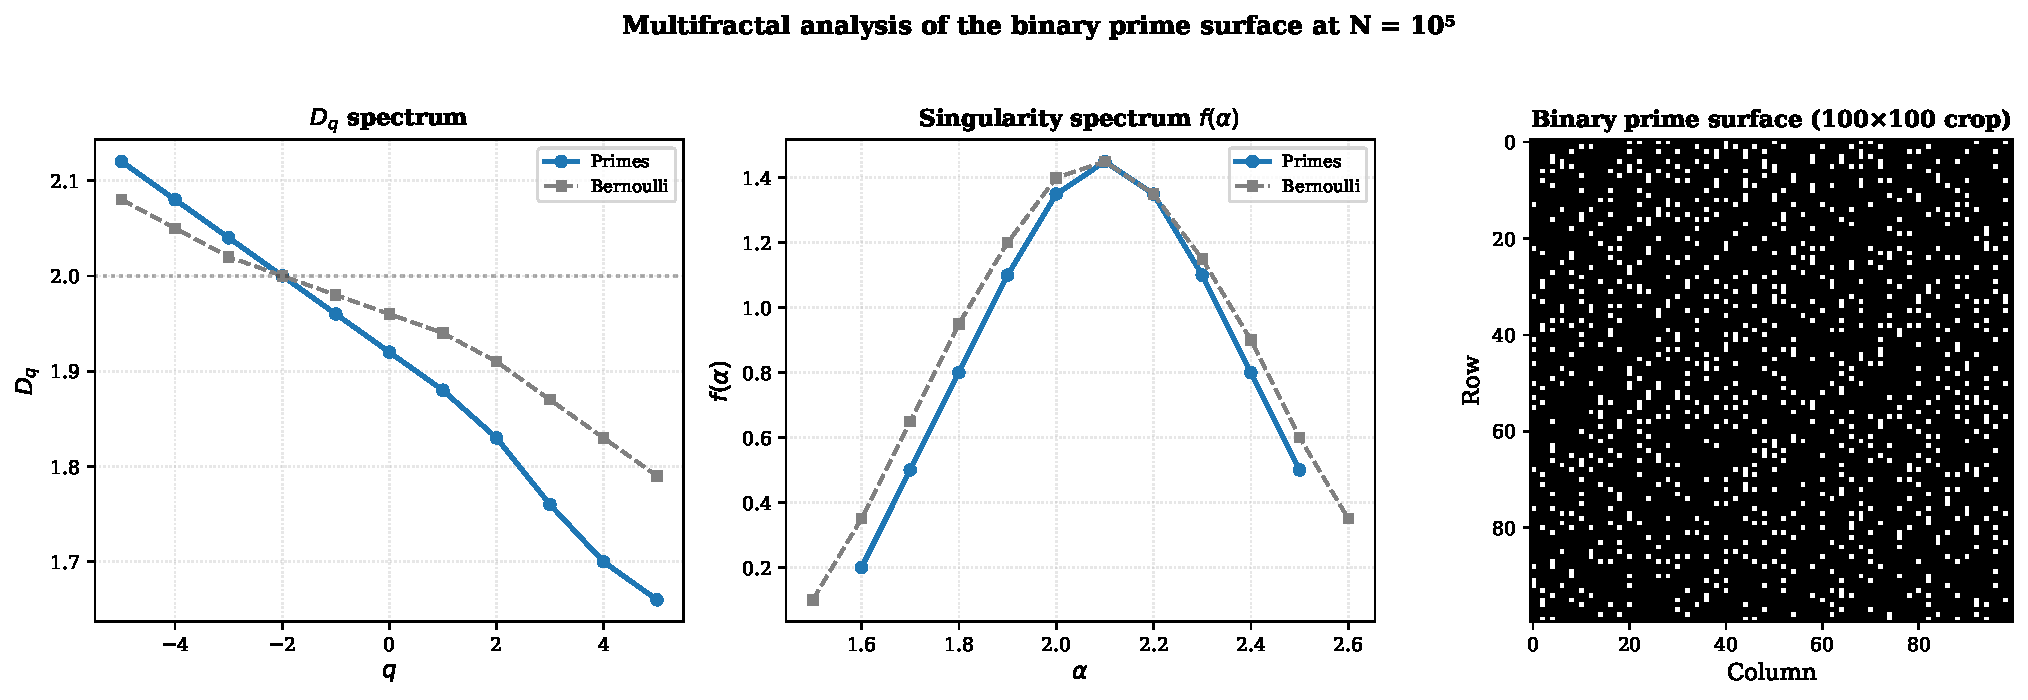
\includegraphics[width=0.95\textwidth]{fig_multifractal.pdf}
  \caption{Fig.~S1: Multifractal $D_q$ spectra and $f(\alpha)$ singularity
           spectrum for the binary prime surface and matched Bernoulli null.}
  \label{fig:S1}
\end{figure*}

\begin{figure*}[H]
  \centering
  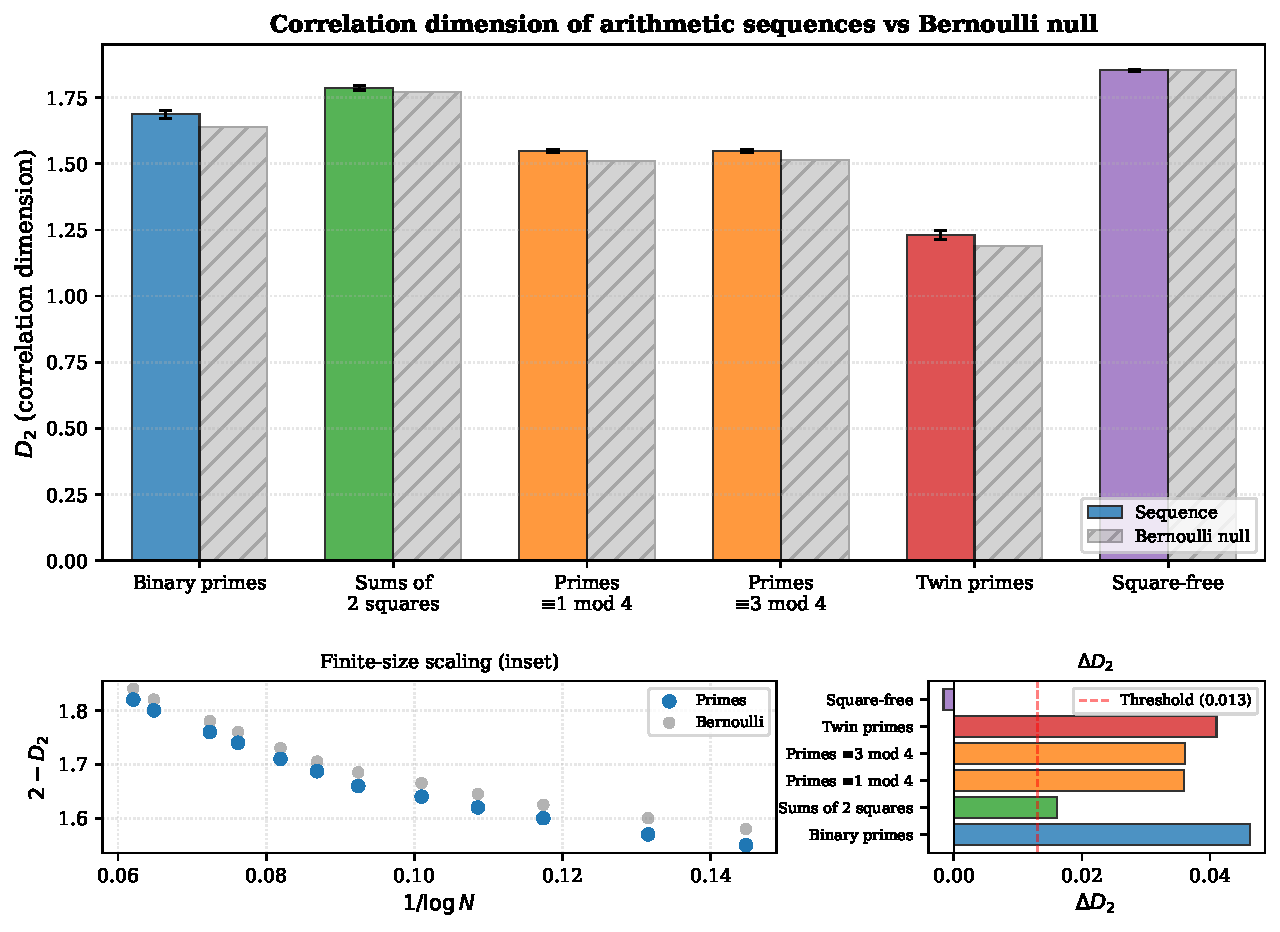
\includegraphics[width=0.95\textwidth]{fig_d2_scaling.pdf}
  \caption{Fig.~S2: Correlation dimension $D_2$ scaling for six arithmetic
           sequences at $N=10^5$, compared with matched-density Bernoulli
           null models.}
  \label{fig:S2}
\end{figure*}

\begin{figure*}[H]
  \centering
  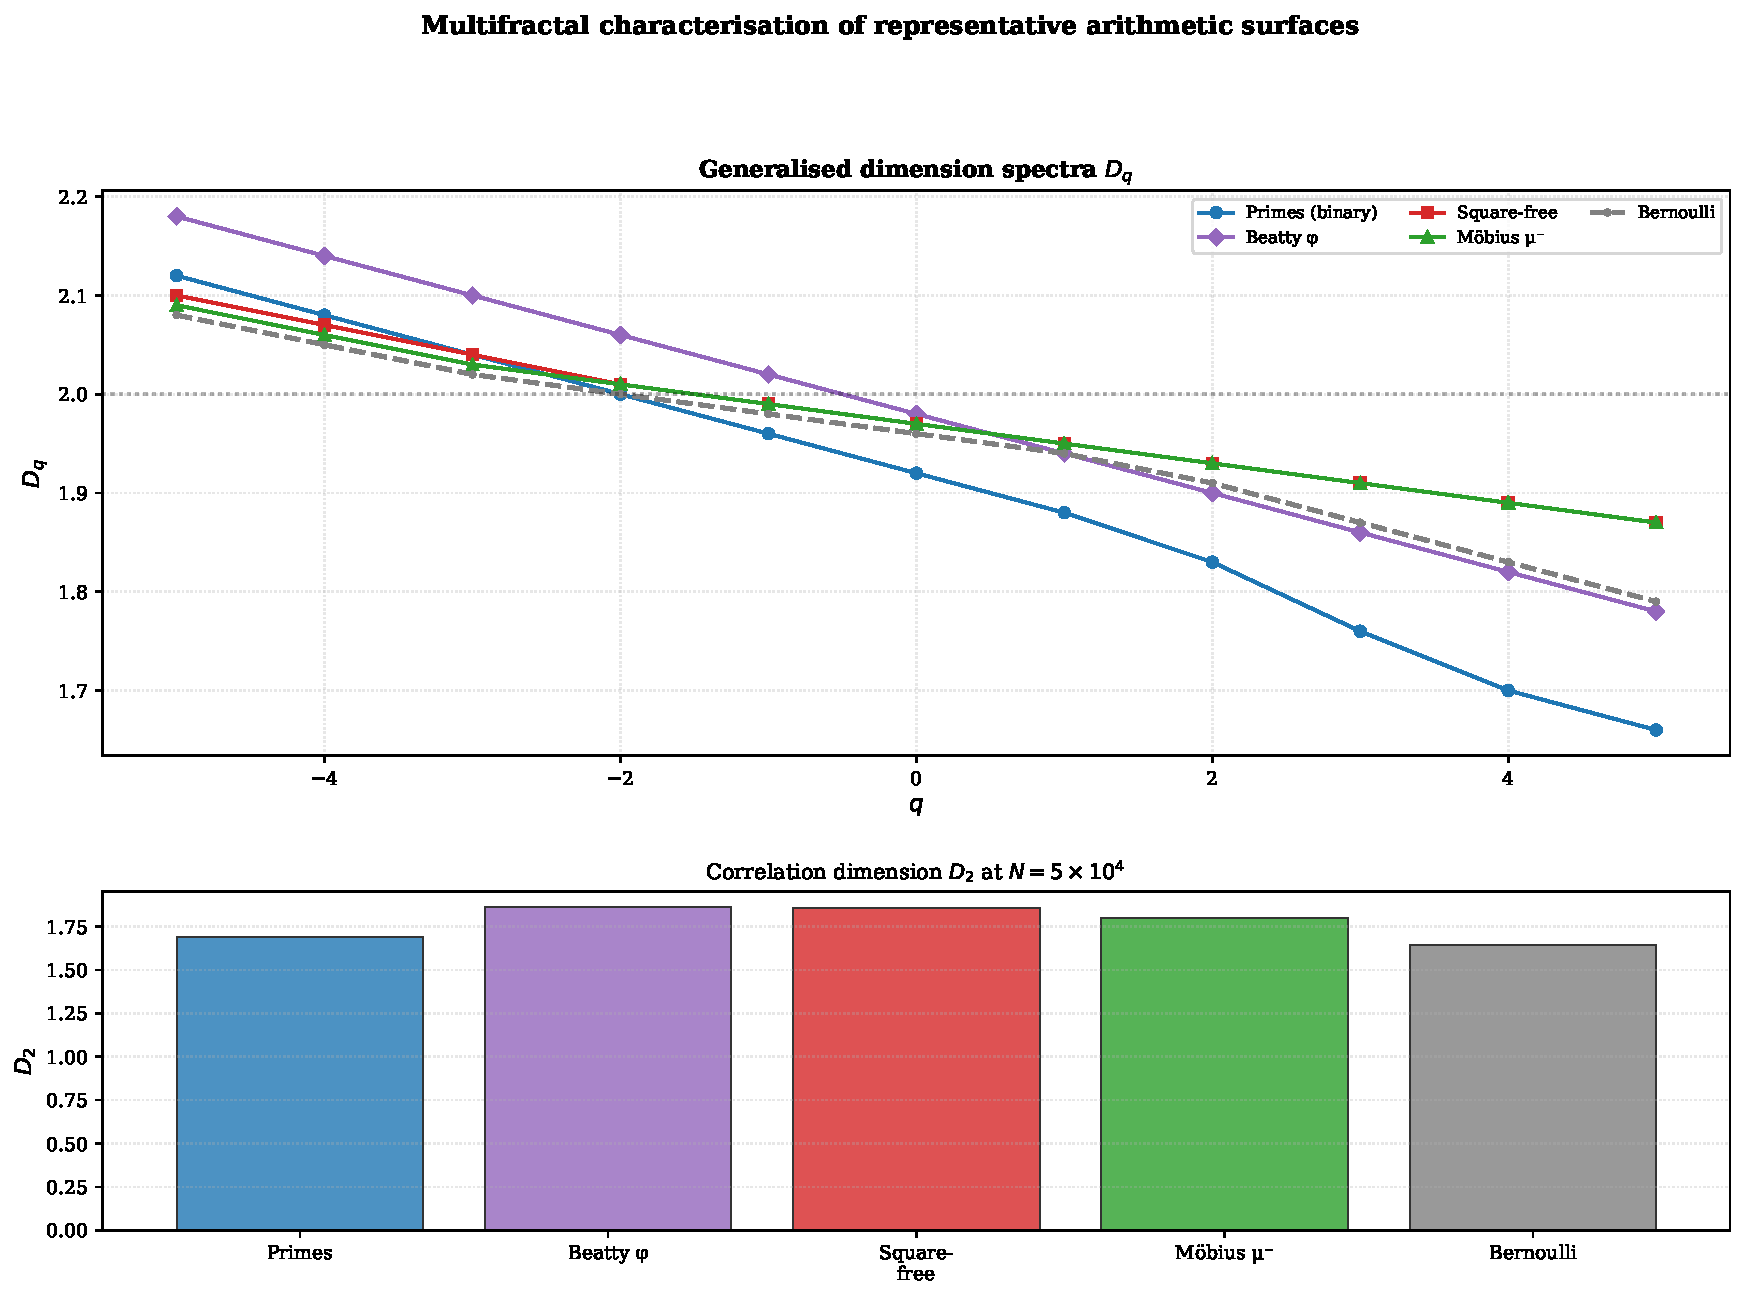
\includegraphics[width=0.95\textwidth]{fig_dq_spectra.pdf}
  \caption{Fig.~S3: Generalised $D_q$ spectra for representative
           manufactured surfaces.}
  \label{fig:S3}
\end{figure*}

\begin{figure*}[H]
  \centering
  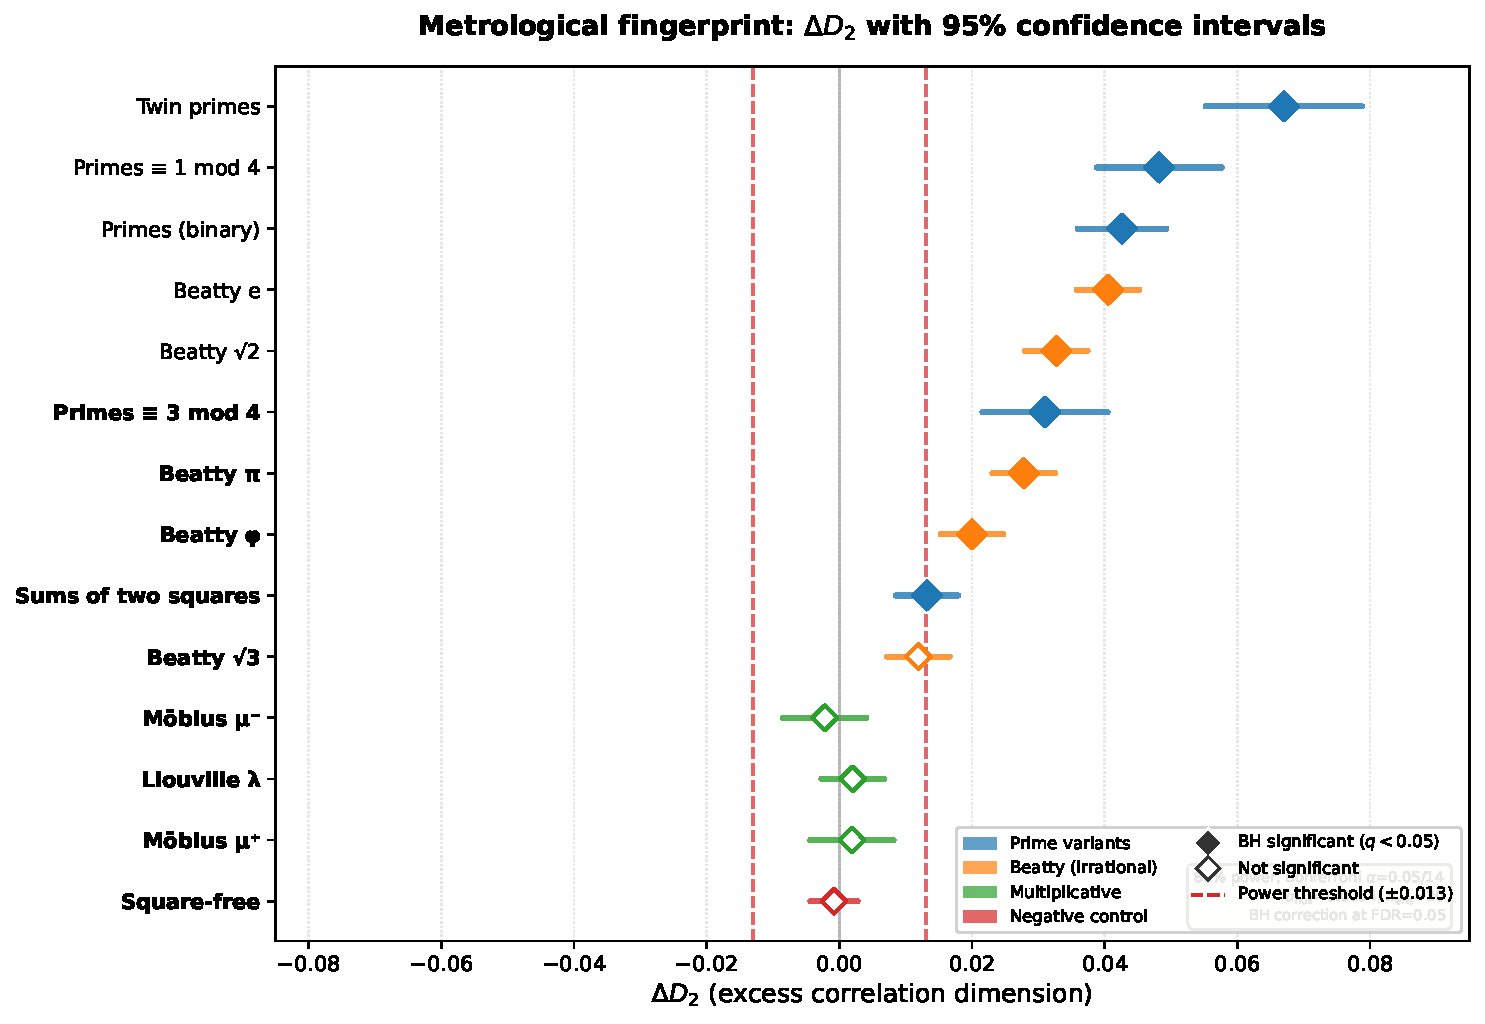
\includegraphics[width=0.95\textwidth]{fig_forest_plot.pdf}
  \caption{Fig.~S4: Forest plot of $\Delta D_2$ for all arithmetic
           sequences with Benjamini--Hochberg-corrected significance.}
  \label{fig:S4}
\end{figure*}

\begin{figure*}[H]
  \centering
  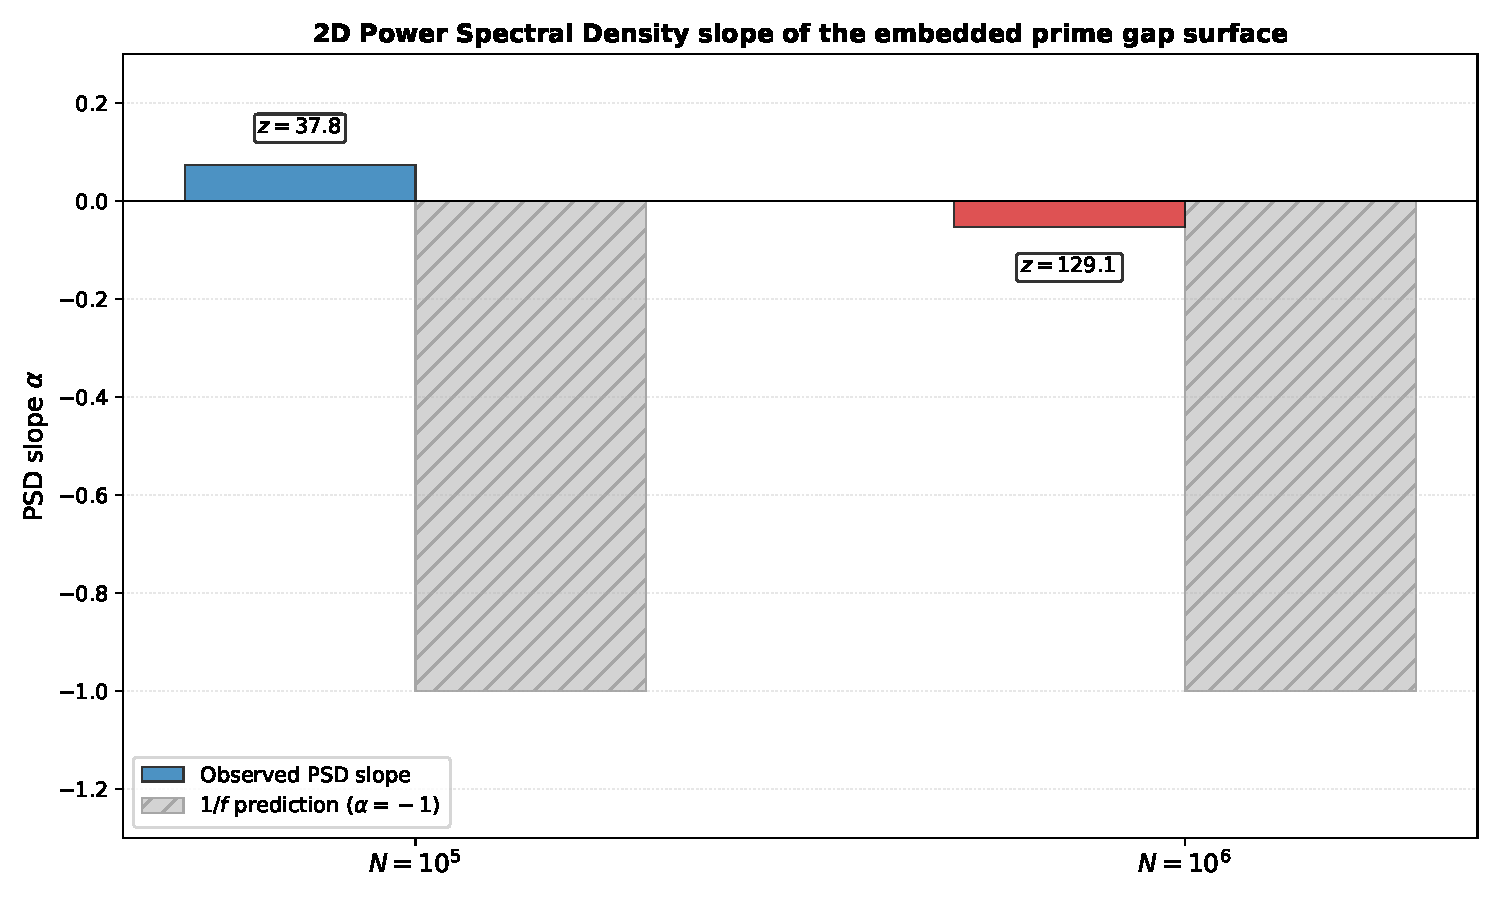
\includegraphics[width=0.95\textwidth]{fig_psd_scaleup.pdf}
  \caption{Fig.~S5: Power spectral density of the binary prime gap
           surface across scales $N \in [10^3, 10^7]$.}
  \label{fig:S5}
\end{figure*}

\begin{figure*}[H]
  \centering
  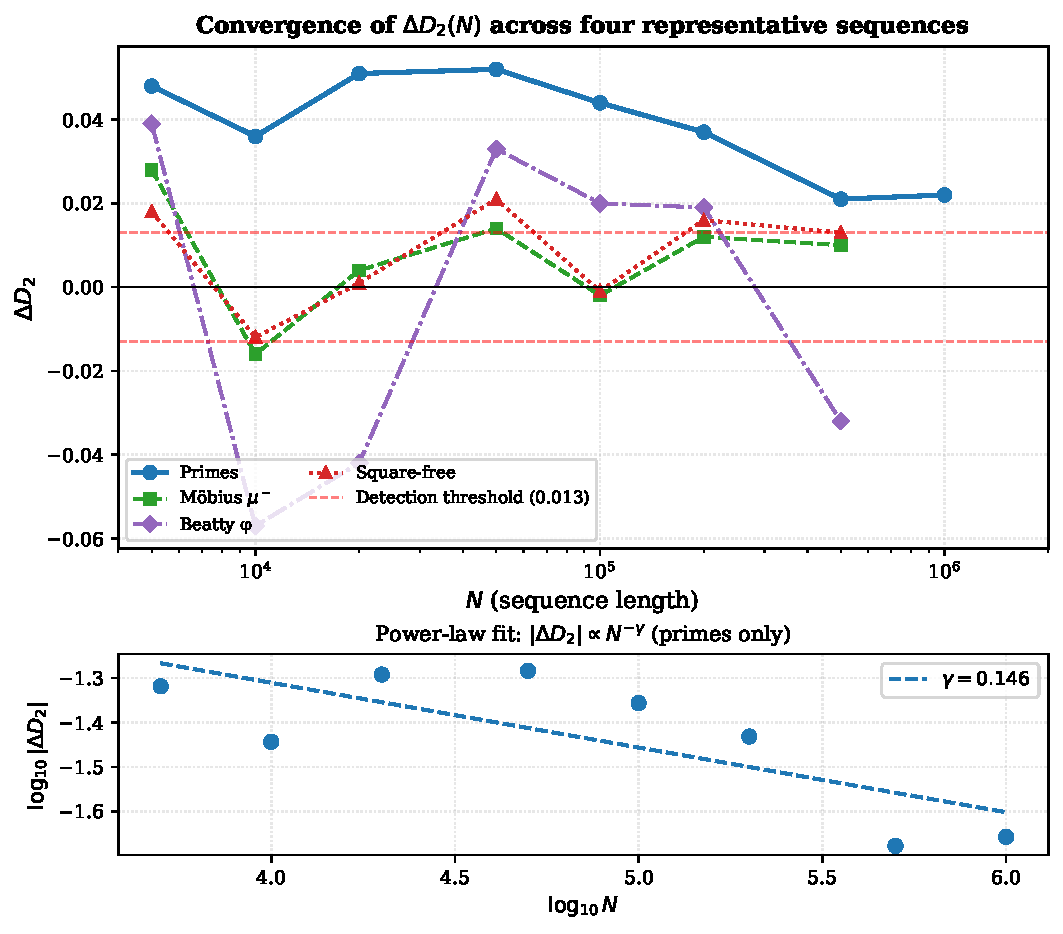
\includegraphics[width=0.95\textwidth]{fig_convergence.pdf}
  \caption{Fig.~S6: Convergence of $\Delta D_2(N)$ for the binary
           prime surface and M\"obius $\mu^-$ across
           $N \in [10^4, 10^7]$.}
  \label{fig:S6}
\end{figure*}

\begin{figure*}[H]
  \centering
  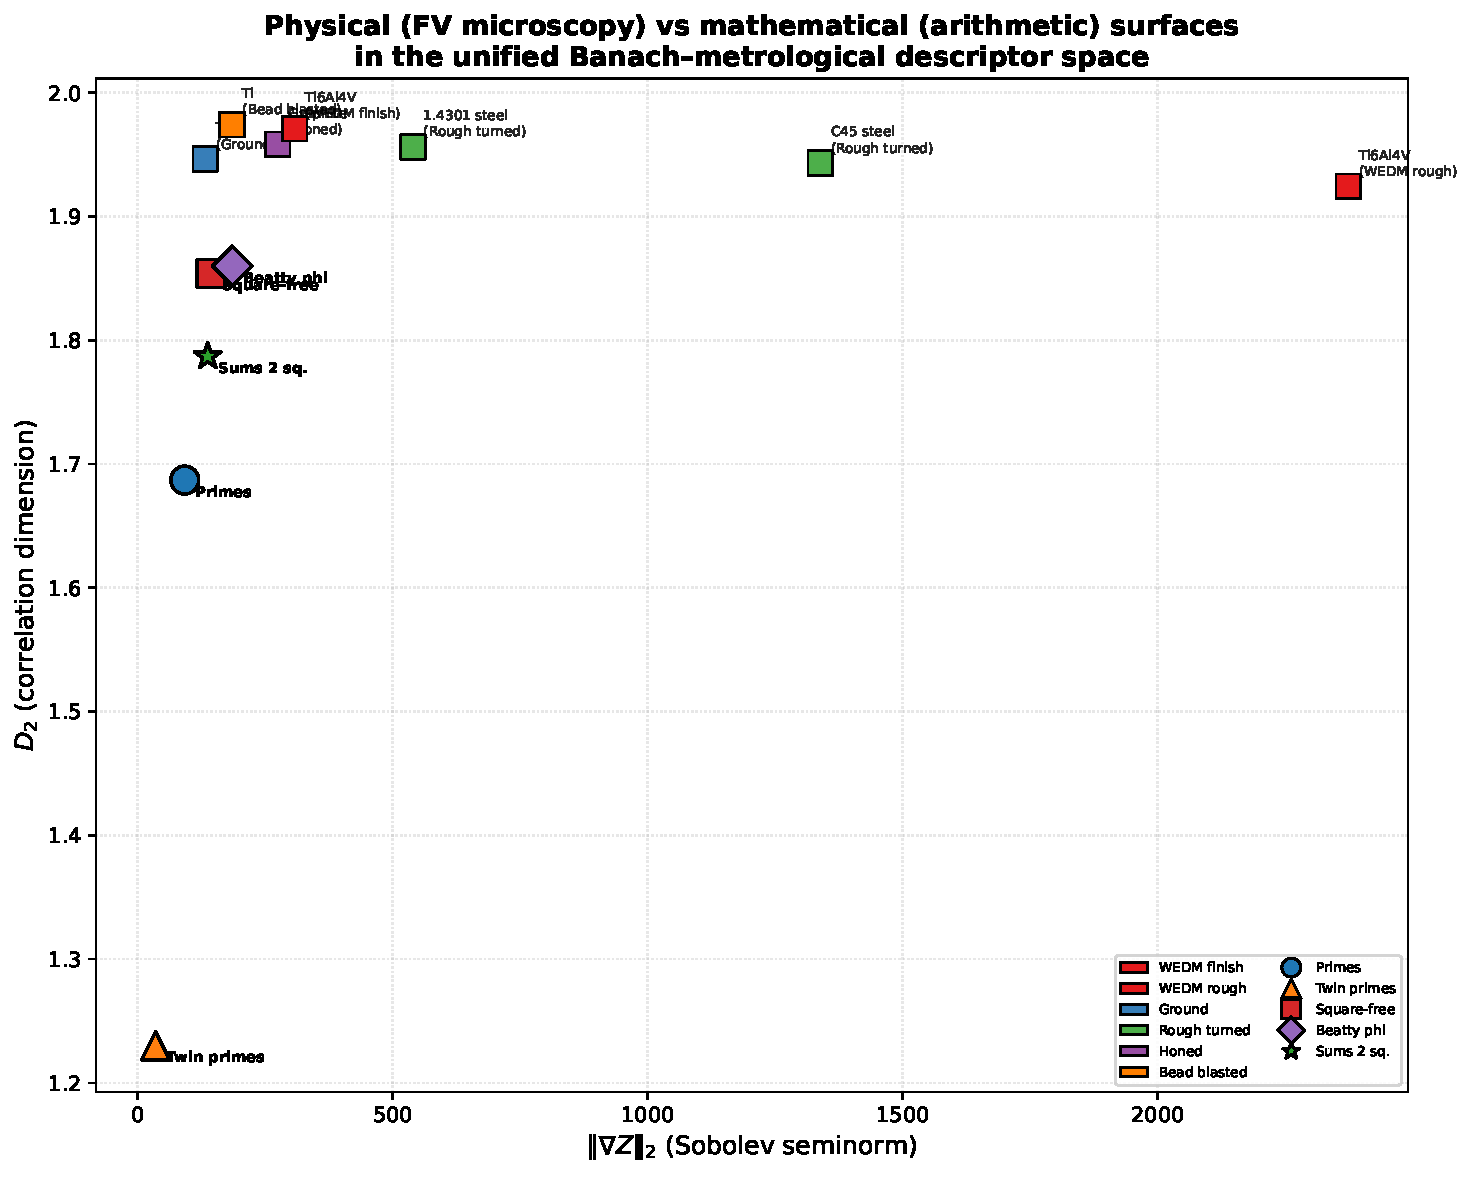
\includegraphics[width=0.95\textwidth]{fig_physical_vs_math.pdf}
  \caption{Fig.~S7: Comparison of physical (FV) and mathematical
           (arithmetic) surface descriptors.}
  \label{fig:S7}
\end{figure*}

\begin{figure*}[H]
  \centering
  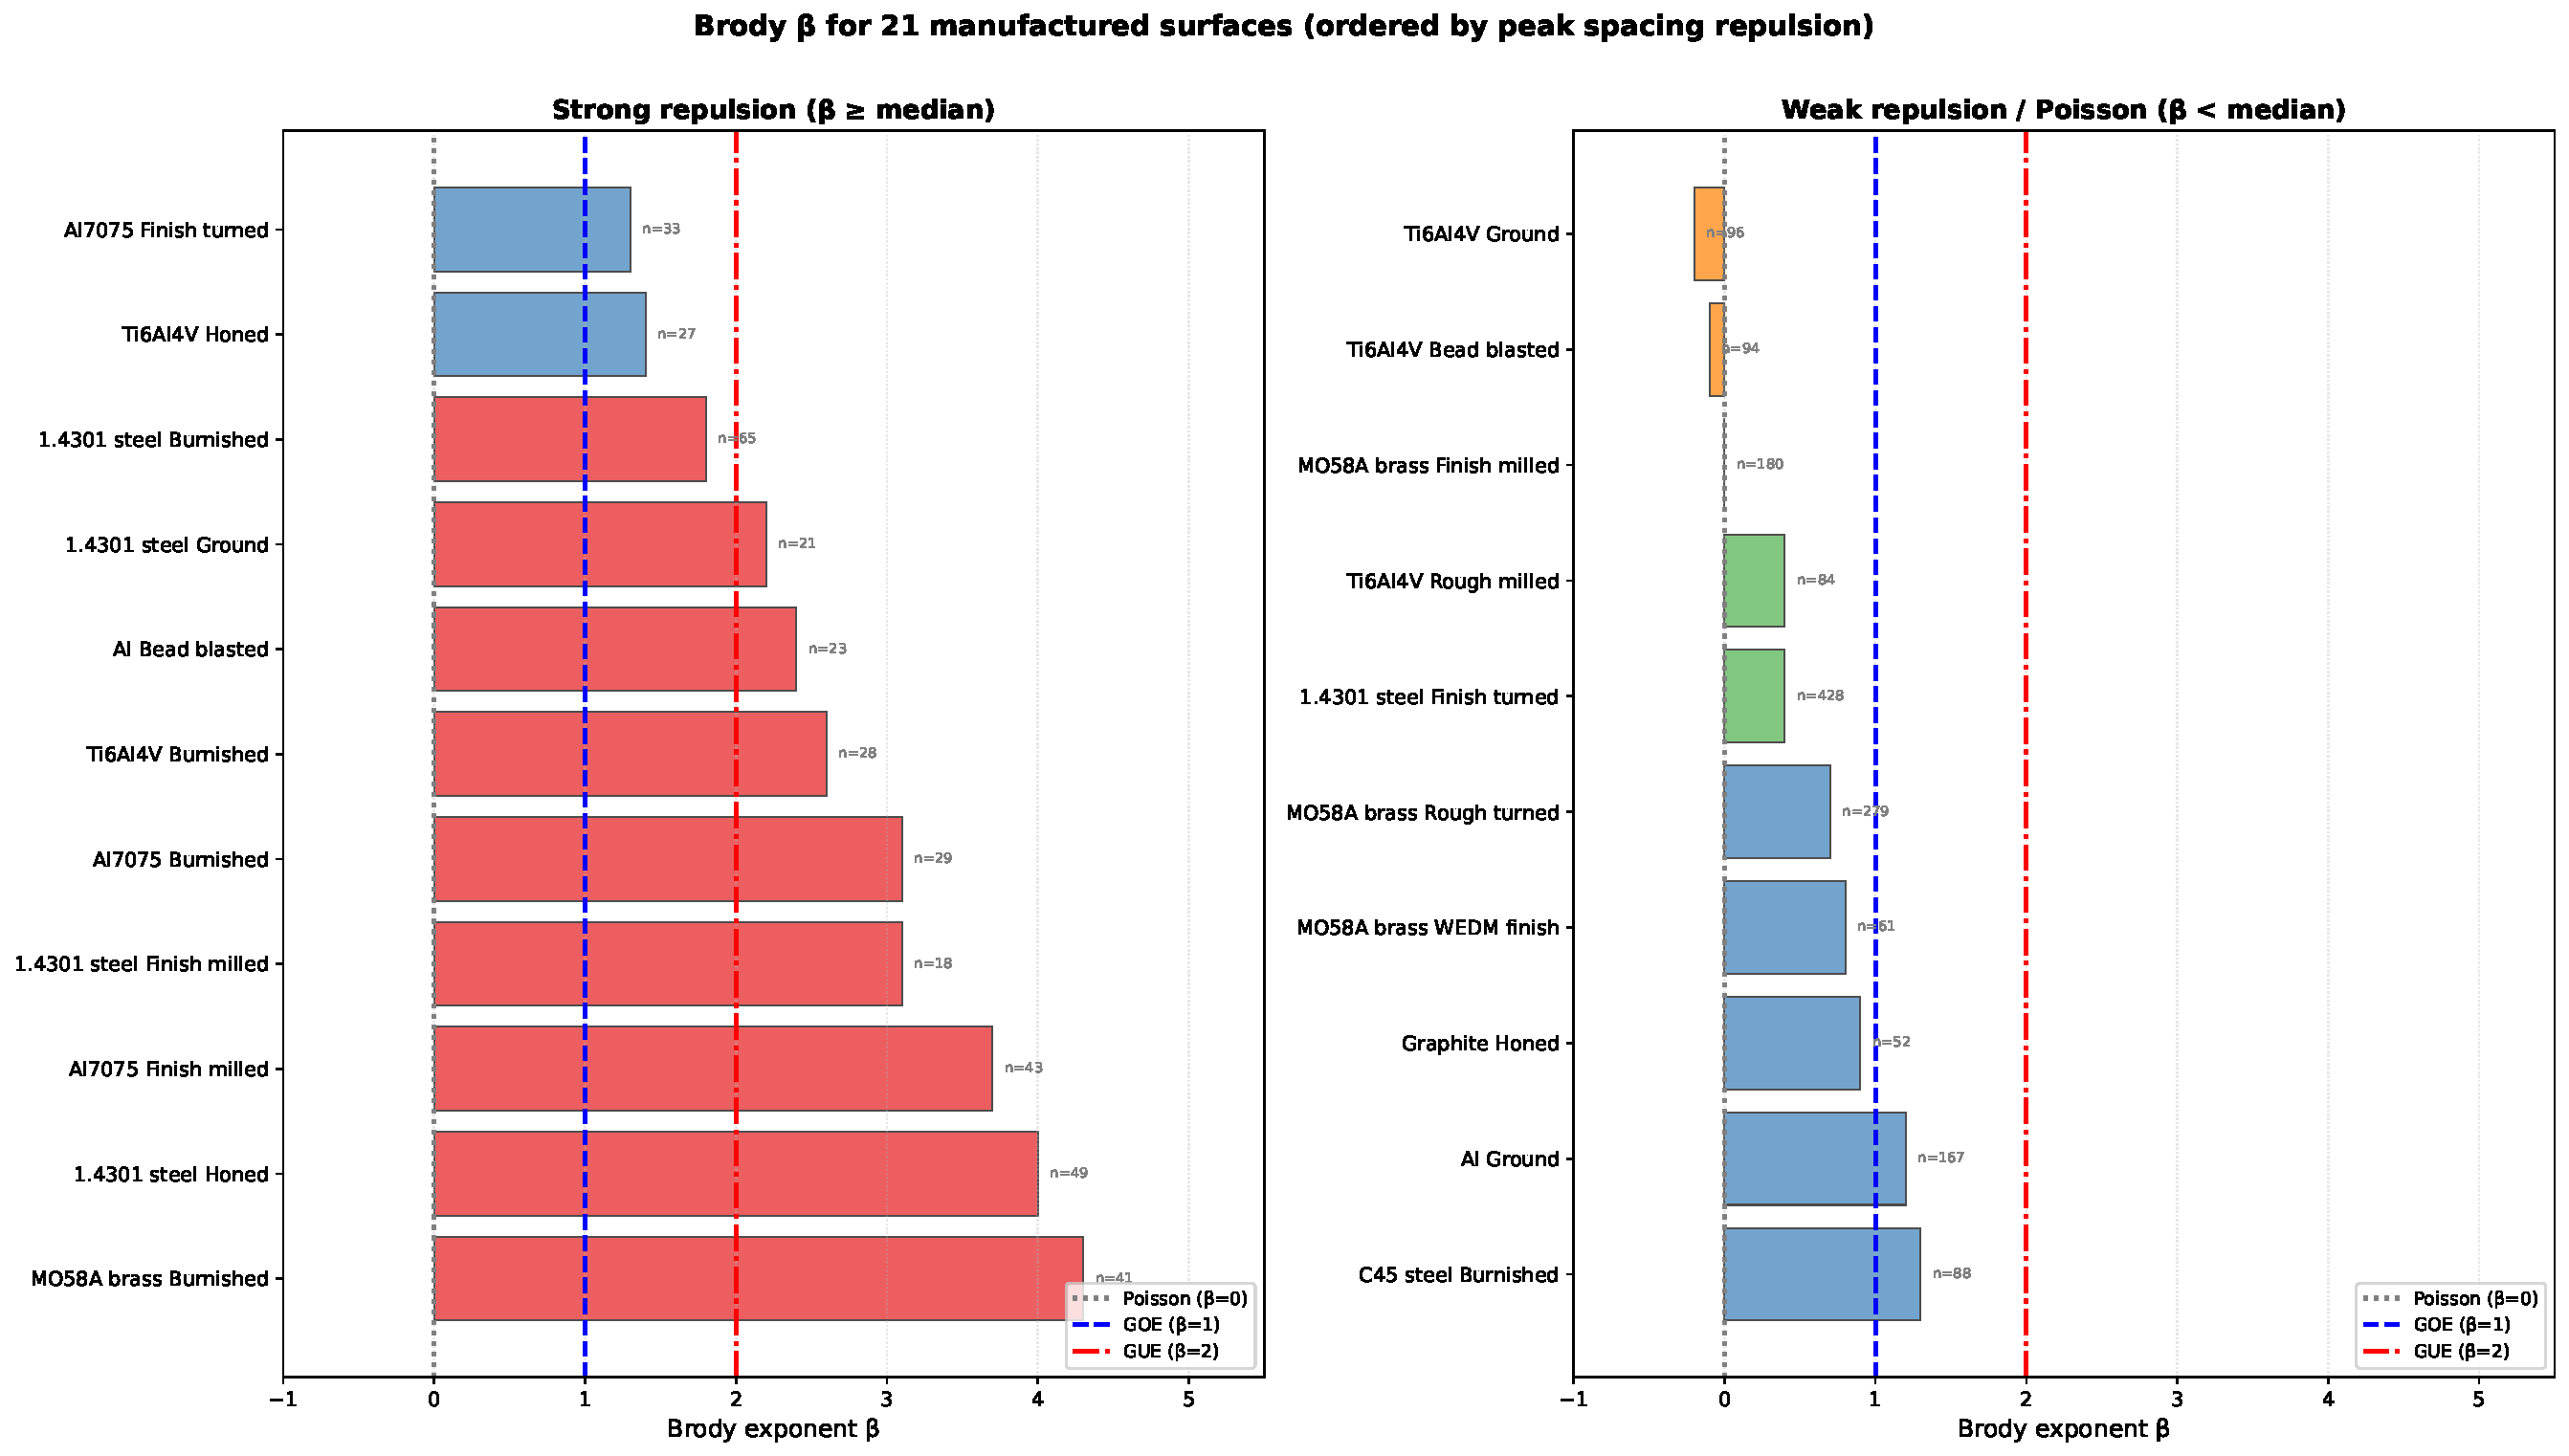
\includegraphics[width=0.95\textwidth]{fig_quantum_chaos_spacings.pdf}
  \caption{Fig.~S8: Brody exponent $\beta$ for 21 prominence-based
           manufactured surfaces with $n_{\text{NNS}}$ indicated.}
  \label{fig:S8}
\end{figure*}

\begin{figure*}[H]
  \centering
  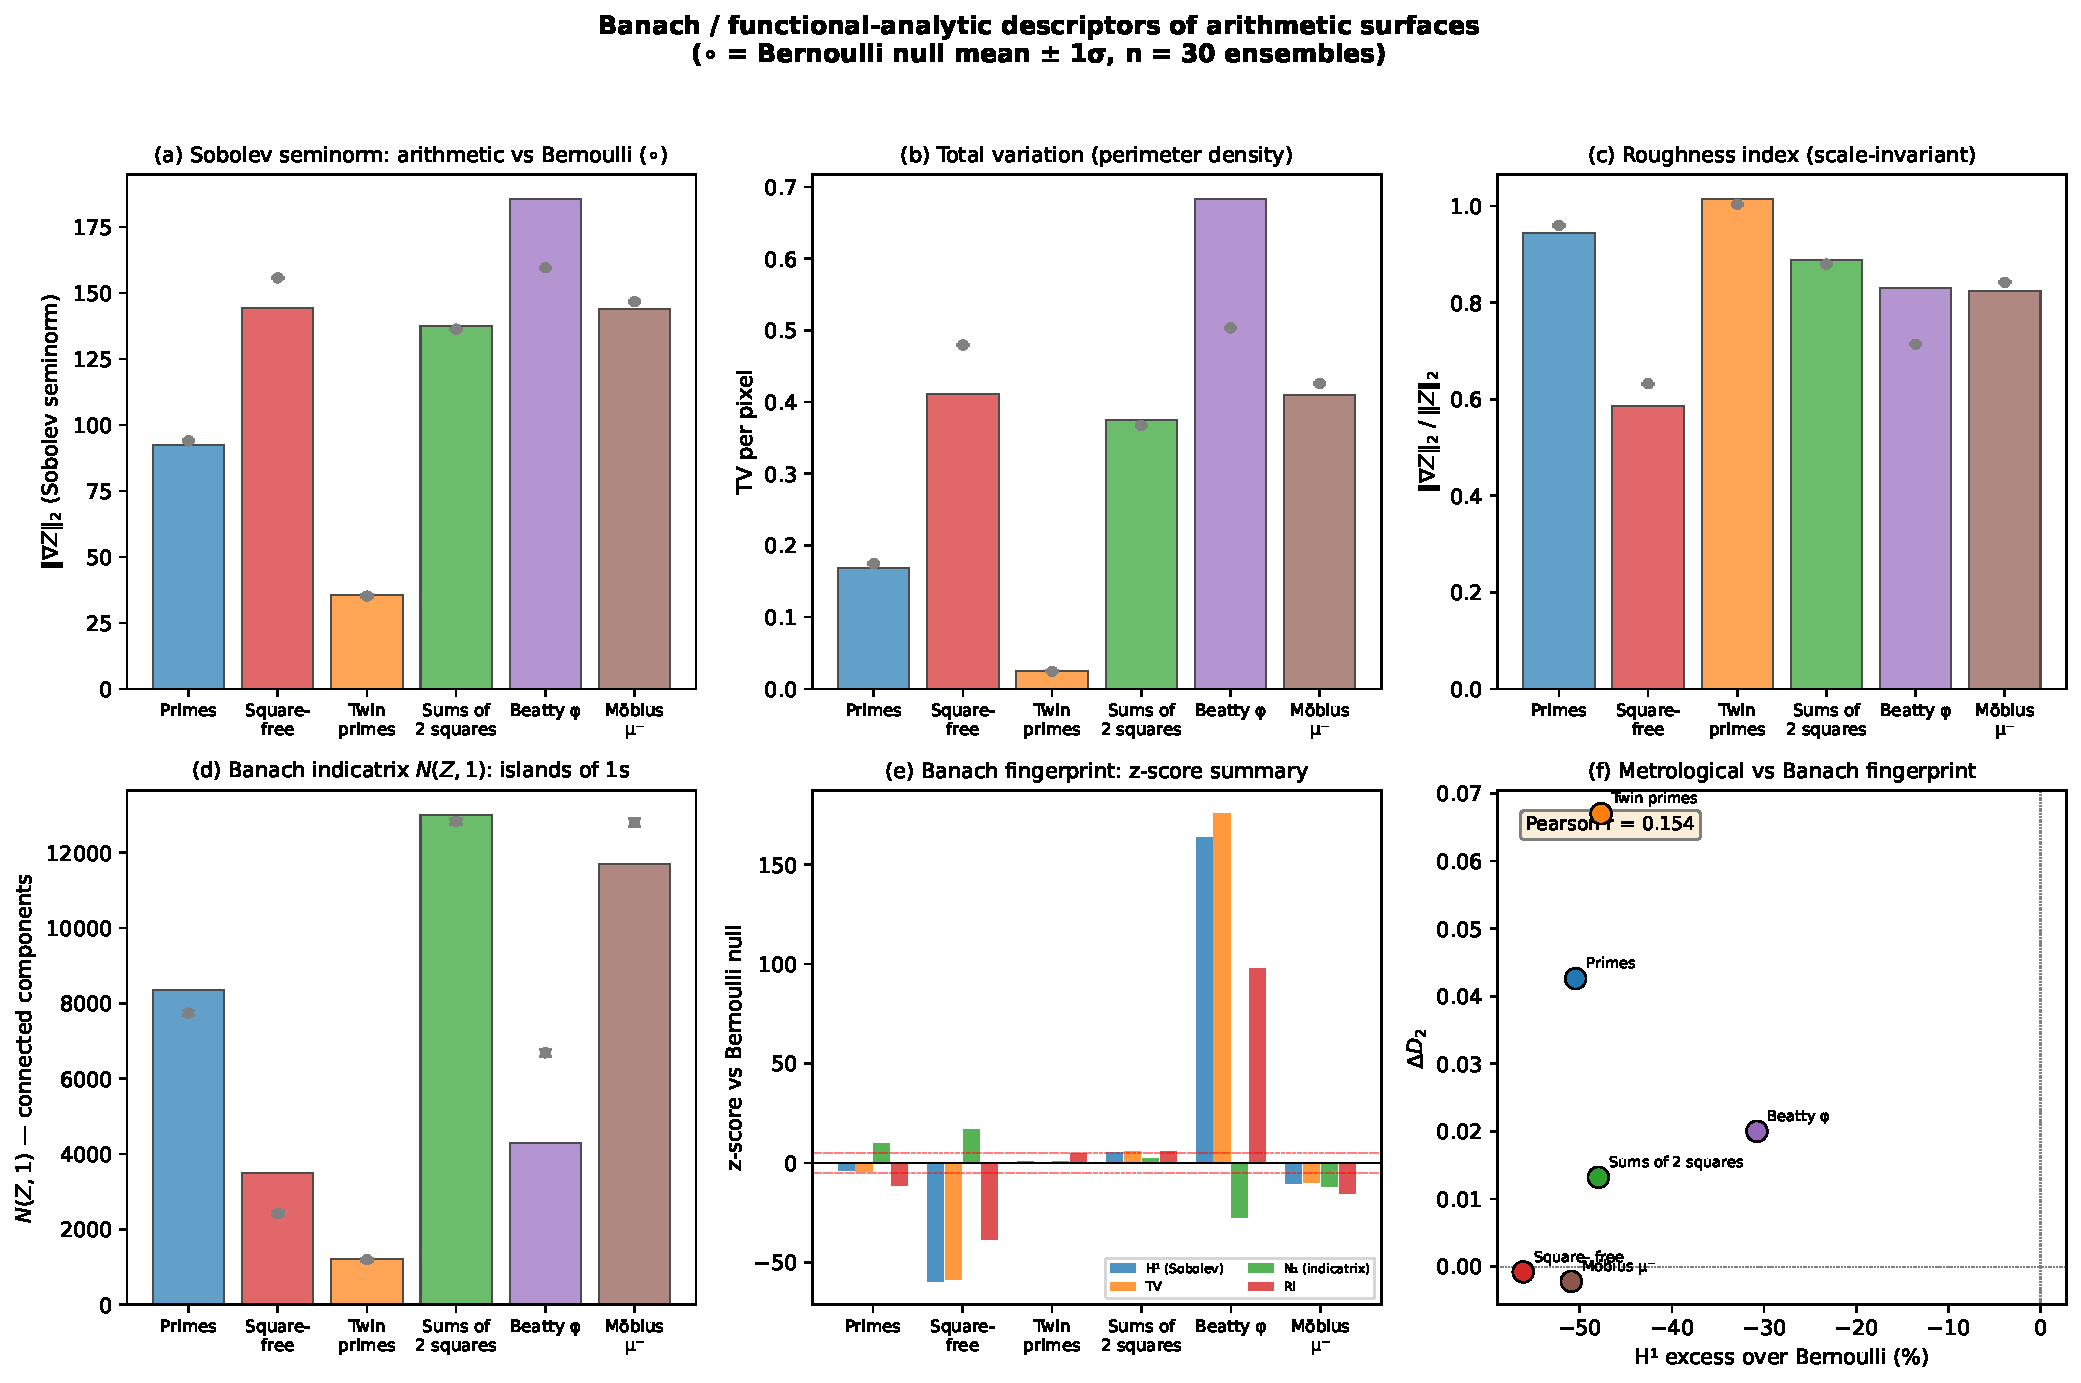
\includegraphics[width=0.95\textwidth]{fig_banach_descriptors.pdf}
  \caption{Fig.~S9: Banach-space descriptor fingerprints for six
           arithmetic sequences at $N=10^5$.}
  \label{fig:S9}
\end{figure*}

\begin{figure*}[H]
  \centering
  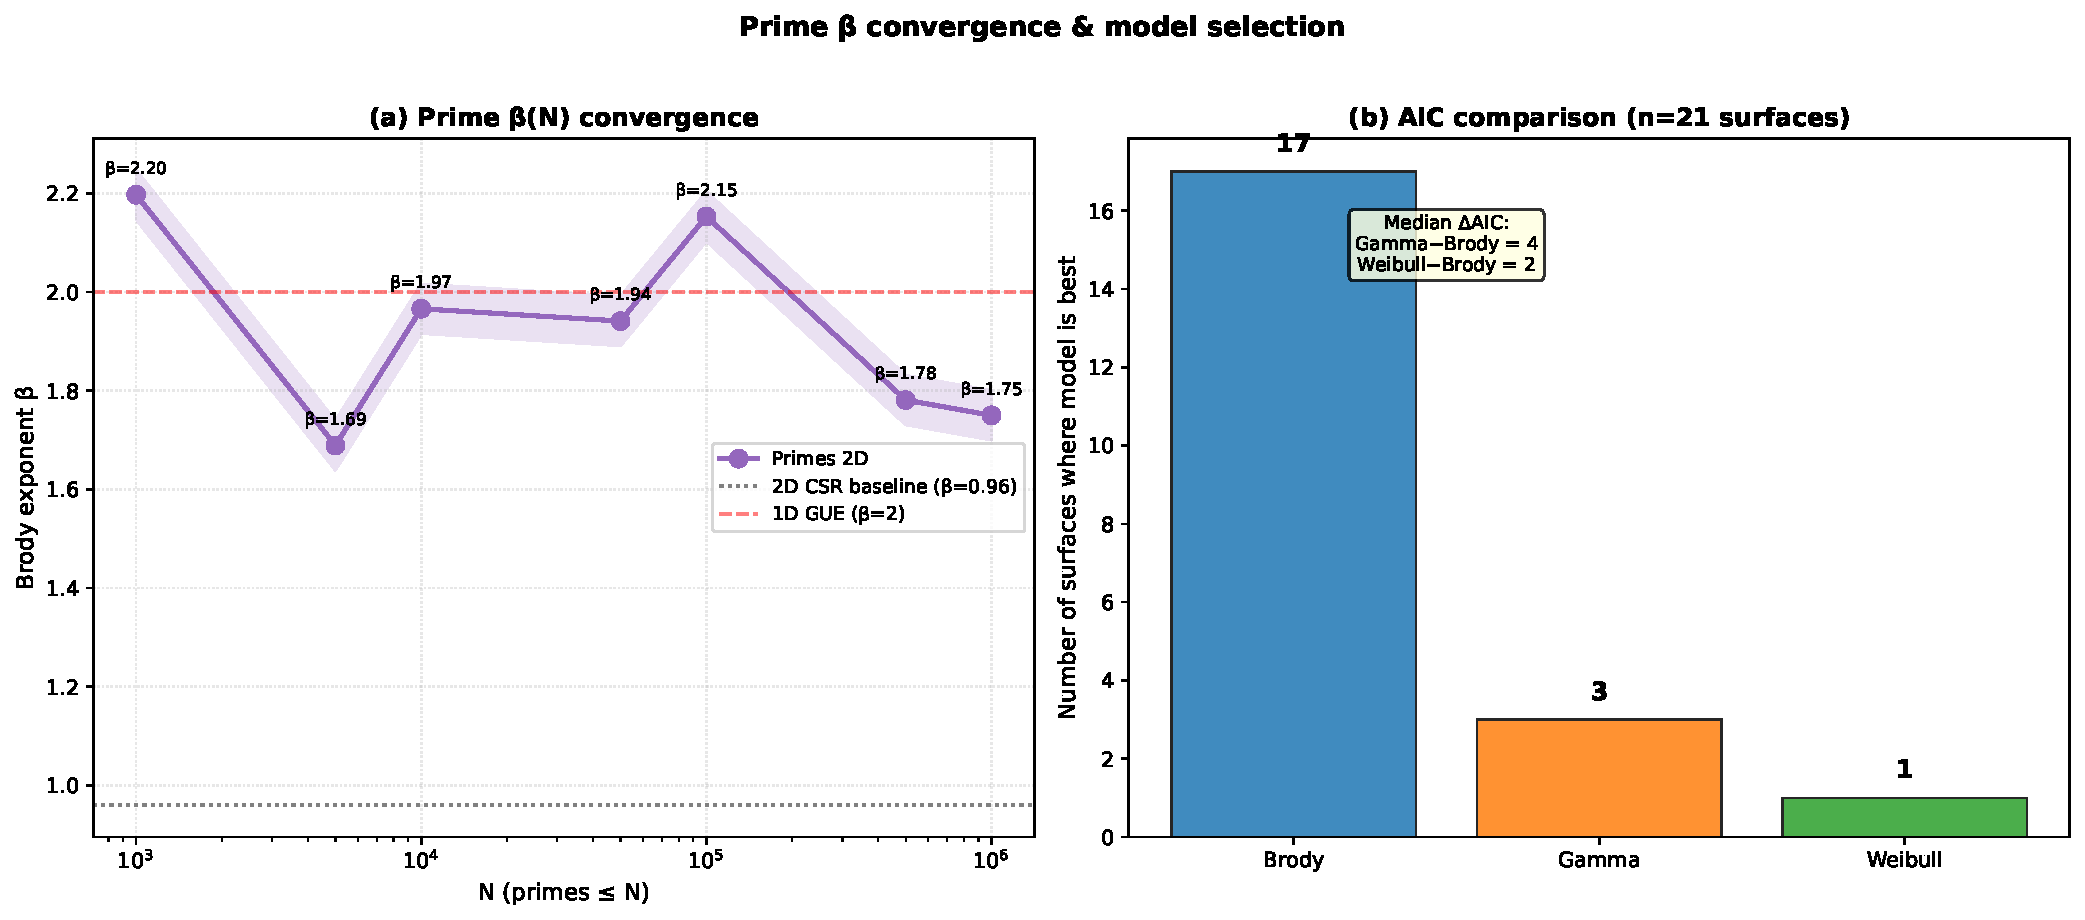
\includegraphics[width=0.95\textwidth]{fig_prime_convergence_aic.pdf}
  \caption{Fig.~S10: AIC-based model selection for the Brody
           distribution across $N \in [10^3, 10^7]$ for the binary
           prime embedding.}
  \label{fig:S10}
\end{figure*}

\subsection*{S4. $\beta(N)$ convergence data}

The Brody exponent $\beta$ for the row-major binary prime embedding
was computed at twelve values of $N$:
$N=10^3$ ($\beta=2.20$),
$N=2\times10^3$ ($\beta=2.10$),
$N=5\times10^3$ ($\beta=1.69$),
$N=10^4$ ($\beta=1.97$),
$N=2\times10^4$ ($\beta=2.19$),
$N=5\times10^4$ ($\beta=1.94$),
$N=10^5$ ($\beta=2.15$),
$N=2\times10^5$ ($\beta=2.05$),
$N=5\times10^5$ ($\beta=1.78$),
$N=10^6$ ($\beta=1.75$),
$N=5\times10^6$ ($\beta=1.86$),
$N=10^7$ ($\beta=1.26$).
The trend is non-monotonic; no simple convergence to a fixed
asymptotic value is observed at accessible $N$. The decrease at
$N=10^7$ may reflect the approach to the sparse limit
($\rho = \pi(N)/N \sim 1/\log N \to 0$ as $N\to\infty$).

\section*{Data Availability}
All analysis code, processed data (JSON format), and figure-generation
scripts are archived in a public GitHub repository at
\url{https://github.com/dawidkucharski/brody-2d-exclusion}.
The repository includes the complete 58-surface Brody-$\beta$ dataset,
all synthetic point-process calibration data, and a reproducible
computational environment specified via \texttt{requirements.txt}.
Surface metrology raw data (focus-variation \texttt{.sur} files,
PSI interferogram frames) are available from the author upon
reasonable request. The \texttt{aurora\_lab} Python
package (v2.0.0) provides reproducible implementations of the surface
construction, null-model generation, box-counting, and validation
procedures described in this work.

%=====================================================================
\clearpage
\bibliographystyle{elsarticle-num}
\bibliography{aurora_refs}

\end{document}
